\chapter{伴随、极限与余极限 I}\label{ch:adjunctions-limits-colimits-I}

直观地说，\trInfinityCategory{}通过添入更高维的态射并弱化复合律，
推广了通常的 1-\trCategory。人们同样可以想象把其他类型的范畴论结构
「∞-化」：添入更高的维度，并弱化诸性质。天真的希望是：那些确立
1-\trCategory{}理论的证明，或许只需处处添一个前缀「∞-」，
便能类似地推广为关于\trInfinityCategory{}的证明。在本章中，
我们使这个梦想成真——至少对一个由基础命题构成的库而言是如此，
这些命题涉及\trEquivalence{}、\trAdjunction{}、\trLimit{}与\trColimit{}%
以及这些概念之间的相互关系。

回顾一下：\trCategory{}、\trFunctor{}与\trNaturalTransformation{}%
构成一个 2-范畴 $\mathcal{C}at$。类似地，任一\trInfinityCosmos{}中的%
\trInfinityCategory{}、\trInfinityFunctor{}与\trInfinityNaturalTransformation{}%
也构成一个 2-范畴，即 §1.4 中引入的该\trInfinityCosmos{}的%
\trHomotopyTwoCategory。事实上，$\mathcal{C}at$ 可以视为某个%
\trHomotopyTwoCategory{}的特例（见第 1 章中的\cref{ex:homotopy-2cat-of-cat}）。
在本章中，我们以 2-范畴论技巧来定义\trInfinityCategory{}之间的%
\trAdjunction{}，以及取值于一个\trInfinityCategory{}的图表的%
\trLimit{}与\trColimit{}，并证明这些概念以预期的方式相互作用。
在\trInfinityCategory{}的\trHomotopyTwoCategory{}中，这就重新得到了
来自 1-\trCategory{}理论的经典结果，某些情形下甚至特殊化为那些标准的证明。
由于这些论证在任何\trHomotopyTwoCategory{}中都同样有效，
我们的证明也只需缀上前缀「∞-」，便同时建立了所期望的推广。

在 §2.1 中，我们把\trInfinityCategory{}之间的\trAdjunction{}定义为%
\trInfinityCategory{}、\trInfinityFunctor{}与\trInfinityNaturalTransformation{}%
的\trHomotopyTwoCategory{}中的一个\trAdjunction。尽管要为这个简单定义的
实质正确性作出辩护尚需一些工夫，但它有一个巨大的优势：关于伴随与%
\trEquivalence{}演算的许多结果，其证明可以「直接取用现成的」——意即
任何对 2-范畴足够稔熟的人可能早已知晓它们。

在 §2.2 中，我们将\trInfinityCategory{}之间的\trAdjunction{}理论
特殊化，以定义并研究一个\trInfinityCategory{}内部的\trInitial{}元素与%
\trTerminal{}元素。本节也充当热身，为更精细的一般理论作预备——
即取值于一个\trInfinityCategory{}的图表的\trLimit{}与\trColimit{}%
的一般理论，那是 §2.3 的主题。最后，在 §2.4 中，我们研究这些概念
之间的相互作用，证明右伴随保持\trLimit{}而左伴随保持\trColimit。

这场讨论尚缺一环，即未谈及与伴随的单位或\trLimit\trCone{}相关联的泛性质。
待我们引入一种合适的「hom \trInfinityCategory{}」以陈述它们之后，
这些内容将在第 4 章重临这些论题时一并纳入。

\providecommand{\Fun}{\operatorname{Fun}}
\providecommand{\Cat}{\mathcal{C}at}
\providecommand{\QCat}{\mathcal{Q}\mathcal{C}at}
\providecommand{\sSet}{s\mathcal{S}et}
\providecommand{\qcOne}{\mathbf{1}}   %
\providecommand{\qcTwo}{\mathbf{2}}   %
\providecommand{\qcThree}{\mathbf{3}} %

\section{\trAdjunction{}与\trEquivalence}\label{sec:adjunctions-equivalences}

在 1.4 节中，我们遇到过 2-\trCategory{}中一对对象之间\emph{\trEquivalence}的定义。
当周围的 2-\trCategory{}是某个\trInfinityCosmos{}的\trHomotopyTwoCategory{}时，
定理 1.4.7 观察到：2-范畴式的\trEquivalence{}概念恰好重新捕捉了整个%
\trInfinityCosmos{}中\trInfinityCategory{}之间的\trEquivalence{}概念。
在我们考察过的每个\trInfinityCosmos{}例子中，\trInfinityCosmos{}里可表示地定义的%
\trEquivalence{}都与该特定模型中呈现的\trInfinityCategory{}之间\trEquivalence{}的
标准概念相重合。\footnote{例如，如题外话 1.2.13 中所述，例 1.2.24 的%
\trInfinityCosmos{}中的\trEquivalence{}重新捕捉了通常\trModelStructure{}中%
\trFibrant--\trCofibrant{}对象之间的\trWeakEquivalence{}。%
}因此，2-范畴式的\trEquivalence{}概念就是\trInfinityCategory{}之间\trEquivalence{}的
「正确」概念。

类似地，2-\trCategory{}中一对对象之间的\emph{\trAdjunction{}}有一个标准定义；把它
诠释到某个\trInfinityCosmos{}中\trInfinityCategory{}、\trFunctor{}与%
\trNaturalTransformation{}的\trHomotopyTwoCategory{}上，将会给出\trInfinityCategory{}%
之间\trAdjunction{}的正确概念。

\begin{definition}[\trAdjunction]\label{def:adjunction}
\trInfinityCategory{}之间的一个\textbf{\trAdjunction}（adjunction）由下列数据构成：

\begin{itemize}
\item 一对\trInfinityCategory $A$ 与 $B$；
\item 一对\trInfinityFunctor{} $u\colon A\to B$ 与 $f\colon B\to A$；以及
\item 一对\trInfinityNaturalTransformation
$\eta\colon\mathrm{id}_B\Rightarrow uf$ 与 $\epsilon\colon fu\Rightarrow\mathrm{id}_A$，
分别称为\textbf{\trUnit}（unit）与\textbf{\trCounit}（counit），
\end{itemize}
使得\trTriangleEqualities{}成立：\footnote{左侧这对粘贴图等式断言了%
\trHomCategory{} $\mathrm{h}\Fun(\mathcal{A},\mathcal{B})$ 中的复合关系
$u\epsilon\cdot\eta u=\mathrm{id}_u$，而右侧等式断言
$\epsilon f\cdot f\eta=\mathrm{id}_f$ 于 $\mathrm{h}\Fun(\mathcal{B},\mathcal{A})$
中。粘贴图的演算在 B.1 节中综述。%
}%
\begin{center}
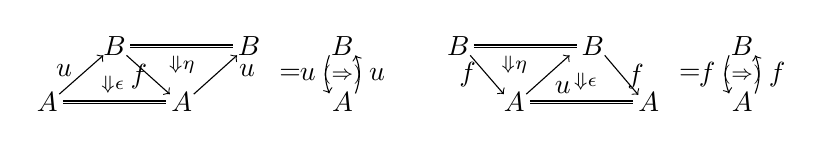
\begin{tikzpicture}[x=1.35em,y=1.35em]
  \node (A1) at (0,0) {$A$};
  \node (A2) at (3.6,0) {$A$};
  \node (B1) at (1.8,1.5) {$B$};
  \node (B2) at (5.4,1.5) {$B$};
  \draw[double] (0.42,0) -- (3.18,0);
  \draw[double] (2.22,1.5) -- (4.98,1.5);
  \draw[->] (0.32,0.22) -- (1.5,1.26);
  \node at (0.45,0.85) {$u$};
  \draw[->] (2.12,1.26) -- (3.28,0.22);
  \node at (2.45,0.68) {$f$};
  \draw[->] (3.92,0.22) -- (5.08,1.26);
  \node at (5.35,0.85) {$u$};
  \node at (1.75,0.48) {$\scriptstyle\Downarrow\epsilon$};
  \node at (3.6,1.0) {$\scriptstyle\Downarrow\eta$};
  \node at (6.5,0.75) {$=$};
  \node (Bs) at (7.9,1.5) {$B$};
  \node (As) at (7.9,0) {$A$};
  \draw[->] (7.55,1.26) to[bend right=20] node[left]{$u$} (7.55,0.24);
  \draw[->] (8.25,0.24) to[bend right=20] node[right]{$u$} (8.25,1.26);
  \node at (7.9,0.75) {$\scriptstyle(\Rightarrow)$};
  \node (B3) at (11.0,1.5) {$B$};
  \node (B4) at (14.6,1.5) {$B$};
  \node (A3) at (12.5,0) {$A$};
  \node (A4) at (16.1,0) {$A$};
  \draw[double] (11.42,1.5) -- (14.18,1.5);
  \draw[double] (12.92,0) -- (15.68,0);
  \draw[->] (11.32,1.26) -- (12.22,0.22);
  \node at (11.25,0.75) {$f$};
  \draw[->] (12.82,0.22) -- (13.98,1.26);
  \node at (13.8,0.4) {$u$};
  \draw[->] (14.92,1.26) -- (15.82,0.2);
  \node at (15.75,0.68) {$f$};
  \node at (12.5,1.0) {$\scriptstyle\Downarrow\eta$};
  \node at (14.4,0.55) {$\scriptstyle\Downarrow\epsilon$};
  \node at (17.2,0.75) {$=$};
  \node (Bt) at (18.6,1.5) {$B$};
  \node (At) at (18.6,0) {$A$};
  \draw[->] (18.25,1.26) to[bend right=20] node[left]{$f$} (18.25,0.24);
  \draw[->] (18.95,0.24) to[bend right=20] node[right]{$f$} (18.95,1.26);
  \node at (18.6,0.75) {$\scriptstyle(\Rightarrow)$};
\end{tikzpicture}
\end{center}
\trFunctor $f$ 称为\textbf{\trLeftAdjoint}（left adjoint），$u$ 称为\textbf{\trRightAdjoint}
（right adjoint）；这一关系在行文中记作 $f\dashv u$，在展示图中则画成
诸如\footnote{有些作者调整伴随图的朝向，使\trLeftAdjoint{}总取某个特定的方向；我们则改用
十字转门符号「$\dashv$」来标明哪个伴随是\trLeftAdjoint{}。}%
的图：
\begin{center}
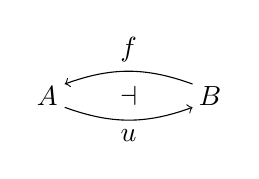
\begin{tikzpicture}[x=1.4em,y=1.4em]
  \node (A) at (0,0) {$A$};
  \node (B) at (4.2,0) {$B$};
  \draw[->] (3.75,0.3) to[bend right=20] node[above]{$f$} (0.45,0.3);
  \node at (2.1,0) {$\dashv$};
  \draw[->] (0.45,-0.3) to[bend right=20] node[below]{$u$} (3.75,-0.3);
\end{tikzpicture}
\end{center}
对\trInfinityCategory{}之间的\trFunctor{}与\trNaturalTransformation{}，
我们通常省略前缀「∞」。
\end{definition}

\begin{digression}[为伴随的 2-范畴式定义辩护]\label{dig:justifying-2categorical-adjunction}
对于觉得\cref{def:adjunction}难以置信——也许简单得让人不敢信任——的读者，
我们愿费少许笔墨作些辩护。率先提议用标准的 2-范畴式定义来定义\trInfinityCategory{}%
之间的\trAdjunction{}的是 Joyal：他在文献 \cite{bib63} 的前言中把\trQuasiCategory{}%
之间的\trAdjunction{}定义为\trHomotopyTwoCategory{} $\mathrm{h}\QCat$ 中的%
\trAdjunction{}。然而这一定义并未被广泛采纳，多数实践者改用 Lurie 的%
\trQuasiCategory{}之间\trAdjunction{}的定义 \cite[\S 5.2]{bib78}，后者取相当
不同的形式。在 F.5 节中，我们将证明：在\trQuasiCategory{}的\trInfinityCosmos{}中，
Joyal 的 2-范畴式\trAdjunction{}定义恰好复原 Lurie 的定义。如第 III 部分所解释的，
例 1.2.24 所描述的 $(\infty,1)$-\trCategory{}的各个模型都「具有同一种范畴论」，
故\cref{def:adjunction}与 $(\infty,1)$-\trCategory{}之间\trAdjunction{}的
共同体共识概念相一致。

在对象为 $(\infty,n)$- 或 $(\infty,\infty)$-\trCategory{}的那些\trInfinityCosmos{}中，
在\trHomotopyTwoCategory{}中定义的\trAdjunction{}是「伪式」（pseudo-style）%
\trAdjunction{}。它们虽不是所能考虑的最一般的\trAdjunction{}——比如，\trTriangleEqualities
关系可以只在相干的不可逆 3-\trCell{}层面成立——但它们是\trAdjunction{}的一个重要
类。\cref{def:adjunction}在一切\trInfinityCosmos{}中都相关的理由之一，在于它与%
\trEquivalence{}的关系——定理 1.4.7 确立这种\trEquivalence{}在实质上是「正确」的——
以及它与即将引入的\trLimit{}与\trColimit{}概念的关系。

最后，一种合理的异议是：\cref{def:adjunction}显得太「低维」，其数据完全落在%
\trHomotopyTwoCategory{}之中而无视\trInfinityCosmos{}中更高维的态射。事实上，
\trInfinityCategory{}之间的任何\trAdjunction{}都可扩充为一份涉及所有维数的%
\emph{\trHomotopyCoherentAdjunction}（homotopy coherent adjunction）数据，而且这种扩充在
同伦意义上唯一 \cite{bib109}。
\end{digression}

\cref{def:adjunction}所给出的\trAdjunction{}定义带有「等式式」的特征：它以
2-\trCategory{}的对象、1-\trCell{}与 2-\trCell{}及其复合来陈述。立即可得：

\begin{lemma}\label{lem:adjunction-preserved-by-2-functor}
2-\trCategory{}中的\trAdjunction{}被任何\trTwoFunctor{}保持。
\end{lemma}

\begin{example}[1-\trCategory{}之间的\trAdjunction]\label{exa:adjunctions-1-categories}
经由\trNerve{}嵌入 $\Cat\hookrightarrow\mathrm{h}\QCat$，1-\trCategory{}之间的任何%
\trAdjunction{}都诱导出其诸\trNerve{}（视作\trQuasiCategory{}）之间的一个%
\trAdjunction{}。
\end{example}

\begin{example}[拓扑\trCategory{}之间的\trAdjunction]\label{exa:adjunctions-topological-categories}
Cordier 的\emph{\trHomotopy{}相干\trNerve}（homotopy coherent nerve）
\cite{bib29,bib30} 定义了一个\trTwoFunctor
$\mathfrak{R}\colon\mathcal{K}an\text{-}\Cat\to\mathrm{h}\QCat$，
它从 Kan 复形\trEnrichedCategory{}、单纯富集\trFunctor{}与单纯%
\trNaturalTransformation{}构成的 2-\trCategory{}出发，映到\trHomotopyTwoCategory{}
$\mathrm{h}\QCat$。如此，拓扑富集的\trAdjunction{}便定义了\trQuasiCategory{}之间的%
\trAdjunction{}。
\end{example}

\begin{example}[Quillen \trAdjunction]\label{exa:quillen-adjunctions}
拓扑富集的\trAdjunction{}相对罕见。更常见的是「在同伦意义下」的拓扑富集%
\trAdjunction{}，例如由（单纯）\trModelCategory{}之间的 Quillen \trAdjunction{}%
所呈现的那类。它们同样定义\trQuasiCategory{}之间的\trAdjunction{}
（见 Mazel-Gee \cite{bib85} 或 \cite[\S 6.2]{bib108}）。
\end{example}

这些例子定义的都是\trQuasiCategory{}之间的\trAdjunction{}，但%
\cref{lem:adjunction-preserved-by-2-functor}也适用于例 1.3.9 的%
\trCosmologicalFunctor{}底下的那些\trTwoFunctor{}，从而把在 $(\infty,1)$-%
\trCategory{}的某个模型中定义的\trAdjunction{}搬运到其余各个模型中定义的%
\trAdjunction{}。而\trTwoFunctor{}对\trAdjunction{}的保持——比如引理 1.4.4 所给出的
那些——也证明了：

\begin{proposition}\label{prop:adjunction-preservation}
给定\trInfinityCategory{}之间的一个\trAdjunction{}：
\begin{center}
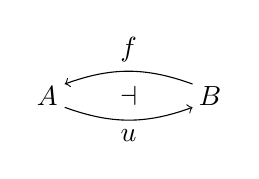
\begin{tikzpicture}[x=1.4em,y=1.4em]
  \node (A) at (0,0) {$A$};
  \node (B) at (4.2,0) {$B$};
  \draw[->] (3.75,0.3) to[bend right=20] node[above]{$f$} (0.45,0.3);
  \node at (2.1,0) {$\dashv$};
  \draw[->] (0.45,-0.3) to[bend right=20] node[below]{$u$} (3.75,-0.3);
\end{tikzpicture}
\end{center}
\begin{enumerate}[label=(\roman*)]
\item 对任何\trInfinityCategory $X$，
\begin{center}
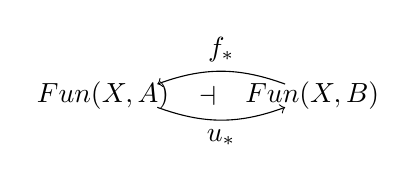
\begin{tikzpicture}[x=1.4em,y=1.4em]
  \node (A) at (0,0) {$\Fun(X,A)$};
  \node (B) at (5.4,0) {$\Fun(X,B)$};
  \draw[->] (4.7,0.3) to[bend right=20] node[above]{$f_\ast$} (1.4,0.3);
  \node at (2.7,0) {$\dashv$};
  \draw[->] (1.4,-0.3) to[bend right=20] node[below]{$u_\ast$} (4.7,-0.3);
\end{tikzpicture}
\end{center}
定义了\trQuasiCategory{}之间的一个\trAdjunction{}；
\item 对任何\trInfinityCategory $X$，
\begin{center}
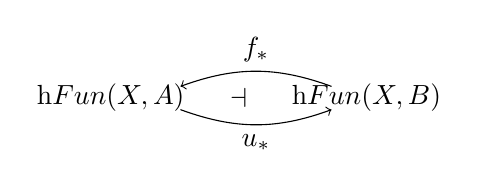
\begin{tikzpicture}[x=1.4em,y=1.4em]
  \node (A) at (0,0) {$\mathrm{h}\Fun(X,A)$};
  \node (B) at (6.6,0) {$\mathrm{h}\Fun(X,B)$};
  \draw[->] (5.7,0.3) to[bend right=20] node[above]{$f_\ast$} (1.8,0.3);
  \node at (3.3,0) {$\dashv$};
  \draw[->] (1.8,-0.3) to[bend right=20] node[below]{$u_\ast$} (5.7,-0.3);
\end{tikzpicture}
\end{center}
定义了\trCategory{}之间的一个\trAdjunction{}；
\item 对任何\trSimplicialSet $U$，
\begin{center}
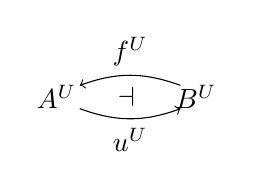
\begin{tikzpicture}[x=1.4em,y=1.4em]
  \node (A) at (0,0) {$A^{U}$};
  \node (B) at (3.6,0) {$B^{U}$};
  \draw[->] (3.2,0.3) to[bend right=20] node[above]{$f^{U}$} (0.6,0.3);
  \node at (1.8,0) {$\dashv$};
  \draw[->] (0.6,-0.3) to[bend right=20] node[below]{$u^{U}$} (3.2,-0.3);
\end{tikzpicture}
\end{center}
定义了\trInfinityCategory{}之间的一个\trAdjunction{}；而且
\item 若周围\trInfinityCosmos{}是\trCartesianClosed{}，则对任何%
\trInfinityCategory $C$，
\begin{center}
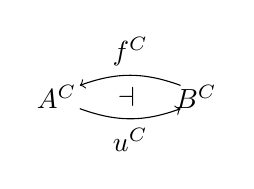
\begin{tikzpicture}[x=1.4em,y=1.4em]
  \node (A) at (0,0) {$A^{C}$};
  \node (B) at (3.6,0) {$B^{C}$};
  \draw[->] (3.2,0.3) to[bend right=20] node[above]{$f^{C}$} (0.6,0.3);
  \node at (1.8,0) {$\dashv$};
  \draw[->] (0.6,-0.3) to[bend right=20] node[below]{$u^{C}$} (3.2,-0.3);
\end{tikzpicture}
\end{center}
定义了\trInfinityCategory{}之间的一个\trAdjunction{}。
\end{enumerate}
\end{proposition}

例如，在 (ii) 中取 $X=1$，便得到\trInfinityCategory $A$ 与 $B$ 的%
\trHomotopyCategory{}之间的一个「导出」\trAdjunction{}（见定义 1.4.11）：
\begin{center}
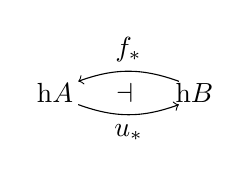
\begin{tikzpicture}[x=1.4em,y=1.4em]
  \node (A) at (0,0) {$\mathrm{h}A$};
  \node (B) at (3.6,0) {$\mathrm{h}B$};
  \draw[->] (3.2,0.3) to[bend right=20] node[above]{$f_\ast$} (0.6,0.3);
  \node at (1.8,0) {$\dashv$};
  \draw[->] (0.6,-0.3) to[bend right=20] node[below]{$u_\ast$} (3.2,-0.3);
\end{tikzpicture}
\end{center}
\begin{proof}
\trHomotopyTwoCategory{} $\mathrm{h}\mathcal{K}$ 的任何\trAdjunction
$f\dashv u$ 都被下列\trTwoFunctor{}保持：
$\Fun(X,-)\colon\mathrm{h}\mathcal{K}\to\mathrm{h}\QCat$、
$\mathrm{h}\Fun(X,-)\colon\mathrm{h}\mathcal{K}\to\Cat$、
$(-)^{U}\colon\mathrm{h}\mathcal{K}\to\mathrm{h}\mathcal{K}$ 与
$(-)^{C}\colon\mathrm{h}\mathcal{K}\to\mathrm{h}\mathcal{K}$。
\end{proof}

\begin{remark}\label{rem:contravariant-adjunction-preservation}
\cref{prop:adjunction-preservation}的每条\trAdjunction{}保持结果都有反变版本；
我们在此详解其中第一条（进一步的讨论见\cref{ex:cotensor-2-functor}）。把%
\trFunctorSpace{}的余域变元固定在任意\trInfinityCategory{} $C\in\mathcal{K}$ 上，
便定义了一个\trTwoFunctor
\[
\Fun(-,C)\colon\mathcal{K}^{op}\longrightarrow\mathrm{h}\QCat
\]
它在 1-\trCell{}上反变而在 2-\trCell{}上共变。\footnote{在 2-\trCategory{}上，
上标「op」表示 1-\trCell{}反转而 2-\trCell{}不反转；上标「co」表示 2-\trCell{}%
反转而 1-\trCell{}不反转；上标「coop」表示 1-\trCell{}与 2-\trCell{}皆反转
（见附录 B 中的\cref{def:op-co-duals}）。%
}这类\trTwoFunctor{}保持\trAdjunction{}，但交换左、\trRightAdjoint{}：比如，给定 $\mathcal{K}$
中的 $f\dashv u$，我们便得到\trFunctorSpace{}之间的一个\trAdjunction{}
\begin{center}
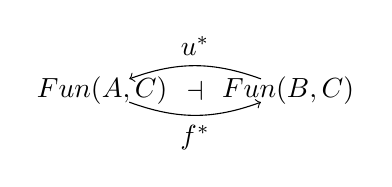
\begin{tikzpicture}[x=1.4em,y=1.4em]
  \node (A) at (0,0) {$\Fun(A,C)$};
  \node (B) at (4.8,0) {$\Fun(B,C)$};
  \draw[->] (4.1,0.3) to[bend right=20] node[above]{$u^{\ast}$} (0.7,0.3);
  \node at (2.4,0) {$\dashv$};
  \draw[->] (0.7,-0.3) to[bend right=20] node[below]{$f^{\ast}$} (4.1,-0.3);
\end{tikzpicture}
\end{center}
\end{remark}

接下来的五个结果都有标准证明，随时可以「现货取用」——只需向恰好驻足近旁的
任意一位 2-范畴理论家讨教即可。唯一的新意在于指出：这些标准论证可以应用到%
\trInfinityCategory{}之间的\trAdjunction{}理论上。

\begin{proposition}\label{prop:adjunctions-compose}
\trAdjunction{}可合成：给定伴随\trFunctor
\begin{center}
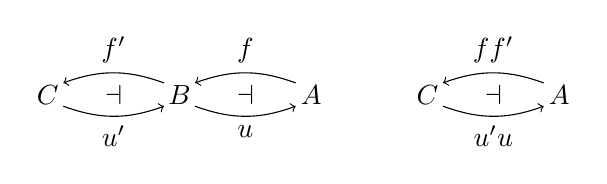
\begin{tikzpicture}[x=1.4em,y=1.4em]
  \node (C) at (0,0) {$C$};
  \node (B) at (3.4,0) {$B$};
  \node (A) at (6.8,0) {$A$};
  \draw[->] (3.0,0.3) to[bend right=20] node[above]{$f'$} (0.4,0.3);
  \node at (1.7,0) {$\dashv$};
  \draw[->] (0.4,-0.3) to[bend right=20] node[below]{$u'$} (3.0,-0.3);
  \draw[->] (6.4,0.3) to[bend right=20] node[above]{$f$} (3.8,0.3);
  \node at (5.1,0) {$\dashv$};
  \draw[->] (3.8,-0.3) to[bend right=20] node[below]{$u$} (6.4,-0.3);
  \node at (8.3,0) {$\rightsquigarrow$};
  \node (C2) at (9.8,0) {$C$};
  \node (A2) at (13.2,0) {$A$};
  \draw[->] (12.8,0.3) to[bend right=20] node[above]{$ff'$} (10.2,0.3);
  \node at (11.5,0) {$\dashv$};
  \draw[->] (10.2,-0.3) to[bend right=20] node[below]{$u'u$} (12.8,-0.3);
\end{tikzpicture}
\end{center}
则复合\trFunctor{}是伴随的。
\end{proposition}
\begin{proof}
记 $\eta\colon\mathrm{id}_B\Rightarrow uf$、$\epsilon\colon fu\Rightarrow\mathrm{id}_A$、
$\eta'\colon\mathrm{id}_C\Rightarrow u'f'$ 与
$\epsilon'\colon f'u'\Rightarrow\mathrm{id}_B$ 为各自的\trUnit{}与\trCounit{}，则粘贴图
\begin{center}
\begin{tikzpicture}[x=1.35em,y=1.35em]
  \node (C1) at (0,2.9) {$C$};
  \node (C2) at (3.6,2.9) {$C$};
  \node (B1) at (1.8,1.45) {$B$};
  \node (B2) at (5.4,1.45) {$B$};
  \node (Ac) at (3.6,0) {$A$};
  \draw[double] (0.42,2.9) -- (3.18,2.9);
  \draw[double] (2.22,1.45) -- (4.98,1.45);
  \draw[->] (0.32,2.66) -- (1.5,1.69);
  \node at (0.35,2.3) {$f'$};
  \draw[->] (2.1,1.69) -- (3.28,2.66);
  \node at (2.35,2.35) {$u'$};
  \draw[->] (2.1,1.2) -- (3.3,0.24);
  \node at (2.0,0.62) {$f$};
  \draw[->] (3.9,0.24) -- (5.08,1.2);
  \node at (5.35,0.62) {$u$};
  \node at (1.8,2.42) {$\scriptstyle\Downarrow\eta'$};
  \node at (3.6,0.97) {$\scriptstyle\Downarrow\eta$};
  \node at (6.0,1.45) {及};
  \node (C3) at (9.2,2.9) {$C$};
  \node (B3) at (7.9,1.45) {$B$};
  \node (B4) at (11.5,1.45) {$B$};
  \node (A3) at (6.7,0) {$A$};
  \node (A4) at (10.3,0) {$A$};
  \draw[double] (8.32,1.45) -- (11.08,1.45);
  \draw[double] (7.12,0) -- (9.88,0);
  \draw[->] (8.22,1.69) -- (8.98,2.66);
  \node at (7.8,2.3) {$u'$};
  \draw[->] (9.42,2.66) -- (10.58,1.69);
  \node at (10.6,2.3) {$f'$};
  \draw[->] (6.92,0.22) -- (7.68,1.21);
  \node at (6.65,0.75) {$u$};
  \draw[->] (8.22,1.21) -- (9.98,0.24);
  \node at (10.1,0.55) {$f$};
  \node at (9.2,1.95) {$\scriptstyle\Downarrow\epsilon'$};
  \node at (8.35,0.5) {$\scriptstyle\Downarrow\epsilon$};
\end{tikzpicture}
\end{center}
定义了 $ff'\dashv u'u$ 的\trUnit{}与\trCounit{}，使得\trTriangleEqualities{}成立：
\begin{center}
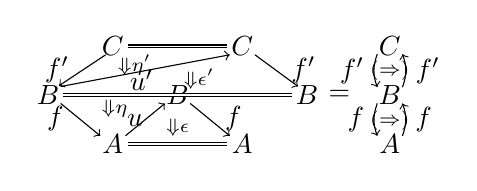
\begin{tikzpicture}[x=1.3em,y=1.22em]
  \node (C1) at (0,4.35) {$C$};
  \node (C2) at (3.6,4.35) {$C$};
  \node (B1) at (-1.8,2.9) {$B$};
  \node (B2) at (1.8,2.9) {$B$};
  \node (B3) at (5.4,2.9) {$B$};
  \node (A1) at (0,1.45) {$A$};
  \node (A2) at (3.6,1.45) {$A$};
  \draw[double] (0.42,4.35) -- (3.18,4.35);
  \draw[double] (-1.38,2.9) -- (4.98,2.9);
  \draw[double] (0.42,1.45) -- (3.18,1.45);
  \draw[->] (-0.2,4.1) -- (-1.5,3.18);
  \node at (-1.55,3.65) {$f'$};
  \draw[->] (-1.45,3.16) -- (3.25,4.1);
  \node at (0.8,3.35) {$u'$};
  \draw[->] (3.95,4.1) -- (5.15,3.16);
  \node at (5.3,3.65) {$f'$};
  \draw[->] (-1.45,2.66) -- (-0.35,1.7);
  \node at (-1.6,2.2) {$f$};
  \draw[->] (0.35,1.7) -- (1.45,2.66);
  \node at (0.62,2.14) {$u$};
  \draw[->] (2.15,2.66) -- (3.25,1.7);
  \node at (3.35,2.2) {$f$};
  \node at (0.6,3.8) {$\scriptstyle\Downarrow\eta'$};
  \node at (2.4,3.38) {$\scriptstyle\Downarrow\epsilon'$};
  \node at (0.05,2.5) {$\scriptstyle\Downarrow\eta$};
  \node at (1.8,1.93) {$\scriptstyle\Downarrow\epsilon$};
  \node at (6.3,2.9) {$=$};
  \node (Cs) at (7.7,4.35) {$C$};
  \node (Bs) at (7.7,2.9) {$B$};
  \node (As) at (7.7,1.45) {$A$};
  \draw[->] (7.35,4.12) to[bend right=20] node[left]{$f'$} (7.35,3.14);
  \draw[->] (8.05,3.14) to[bend right=20] node[right]{$f'$} (8.05,4.12);
  \node at (7.7,3.62) {$\scriptstyle(\Rightarrow)$};
  \draw[->] (7.35,2.66) to[bend right=20] node[left]{$f$} (7.35,1.7);
  \draw[->] (8.05,1.7) to[bend right=20] node[right]{$f$} (8.05,2.66);
  \node at (7.7,2.16) {$\scriptstyle(\Rightarrow)$};
\end{tikzpicture}
\end{center}
\begin{center}
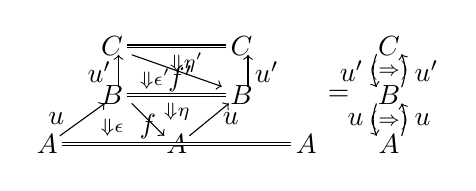
\begin{tikzpicture}[x=1.3em,y=1.22em]
  \node (C1) at (0,4.35) {$C$};
  \node (C2) at (3.6,4.35) {$C$};
  \node (B1) at (0,2.9) {$B$};
  \node (B2) at (3.6,2.9) {$B$};
  \node (A1) at (-1.8,1.45) {$A$};
  \node (A2) at (1.8,1.45) {$A$};
  \node (A3) at (5.4,1.45) {$A$};
  \draw[double] (0.42,4.35) -- (3.18,4.35);
  \draw[double] (0.42,2.9) -- (3.18,2.9);
  \draw[double] (-1.38,1.45) -- (4.98,1.45);
  \draw[->] (0.18,3.14) -- (0.18,4.1);
  \node at (-0.35,3.6) {$u'$};
  \draw[->] (0.55,4.1) -- (3.05,3.16);
  \node at (1.9,3.4) {$f'$};
  \draw[->] (3.78,3.14) -- (3.78,4.1);
  \node at (4.3,3.6) {$u'$};
  \draw[->] (-1.45,1.7) -- (-0.2,2.66);
  \node at (-1.55,2.2) {$u$};
  \draw[->] (0.55,2.66) -- (1.45,1.7);
  \node at (1.0,1.98) {$f$};
  \draw[->] (2.15,1.7) -- (3.25,2.66);
  \node at (3.3,2.2) {$u$};
  \node at (1.2,3.38) {$\scriptstyle\Downarrow\epsilon'$};
  \node at (2.07,3.87) {$\scriptstyle\Downarrow\eta'$};
  \node at (0.0,1.93) {$\scriptstyle\Downarrow\epsilon$};
  \node at (1.8,2.42) {$\scriptstyle\Downarrow\eta$};
  \node at (6.3,2.9) {$=$};
  \node (Cs) at (7.7,4.35) {$C$};
  \node (Bs) at (7.7,2.9) {$B$};
  \node (As) at (7.7,1.45) {$A$};
  \draw[->] (7.35,4.12) to[bend right=20] node[left]{$u'$} (7.35,3.14);
  \draw[->] (8.05,3.14) to[bend right=20] node[right]{$u'$} (8.05,4.12);
  \node at (7.7,3.62) {$\scriptstyle(\Rightarrow)$};
  \draw[->] (7.35,2.66) to[bend right=20] node[left]{$u$} (7.35,1.7);
  \draw[->] (8.05,1.7) to[bend right=20] node[right]{$u$} (8.05,2.66);
  \node at (7.7,2.16) {$\scriptstyle(\Rightarrow)$};
\end{tikzpicture}
\end{center}
\end{proof}

给定\trFunctor{}的伴随在同构意义下唯一：

\begin{proposition}[伴随的唯一性]\label{prop:uniqueness-of-adjoints}
\begin{enumerate}[label=(\roman*)]
\item 若 $f\dashv u$ 且 $f'\dashv u$，则 $f\cong f'$。
\item 反之，若 $f\dashv u$ 且 $f\cong f'$，则 $f'\dashv u$。
\end{enumerate}
\end{proposition}
\begin{proof}
记 $\eta\colon\mathrm{id}_B\Rightarrow uf$、$\epsilon\colon fu\Rightarrow\mathrm{id}_A$、
$\eta'\colon\mathrm{id}_B\Rightarrow uf'$ 与
$\epsilon'\colon f'u\Rightarrow\mathrm{id}_A$ 为各自的\trUnit{}与\trCounit{}，则粘贴图
\begin{center}
\begin{tikzpicture}[x=1.35em,y=1.35em]
  \node (B1) at (0,1.5) {$B$};
  \node (B2) at (3.6,1.5) {$B$};
  \node (A1) at (1.8,0) {$A$};
  \node (A2) at (5.4,0) {$A$};
  \draw[double] (0.42,1.5) -- (3.18,1.5);
  \draw[double] (2.22,0) -- (4.98,0);
  \draw[->] (0.32,1.26) -- (1.52,0.22);
  \node at (0.45,0.75) {$f'$};
  \draw[->] (2.12,0.22) -- (3.28,1.26);
  \node at (3.0,0.4) {$u$};
  \draw[->] (3.92,1.26) -- (5.08,0.22);
  \node at (5.15,0.75) {$f$};
  \node at (1.8,1.0) {$\scriptstyle\Downarrow\eta'$};
  \node at (3.75,0.62) {$\scriptstyle\Downarrow\epsilon$};
  \node at (6.6,0.75) {与};
  \node (B3) at (7.5,1.5) {$B$};
  \node (B4) at (11.1,1.5) {$B$};
  \node (A3) at (9.3,0) {$A$};
  \node (A4) at (12.9,0) {$A$};
  \draw[double] (7.92,1.5) -- (10.68,1.5);
  \draw[double] (9.72,0) -- (12.48,0);
  \draw[->] (7.82,1.26) -- (9.02,0.22);
  \node at (7.95,0.75) {$f$};
  \draw[->] (9.62,0.22) -- (10.78,1.26);
  \node at (10.5,0.4) {$u$};
  \draw[->] (11.42,1.26) -- (12.62,0.22);
  \node at (12.75,0.6) {$f'$};
  \node at (9.3,1.0) {$\scriptstyle\Downarrow\eta$};
  \node at (11.25,0.62) {$\scriptstyle\Downarrow\epsilon'$};
\end{tikzpicture}
\end{center}
定义了 2-\trCell{} $f\Rightarrow f'$ 与 $f'\Rightarrow f$。复合
$f\Rightarrow f'\Rightarrow f$ 与 $f'\Rightarrow f\Rightarrow f'$ 则通过把这两张图
从某一侧或另一侧水平地粘贴起来而计算。对\trAdjunction{} $f\dashv u$ 与
$f'\dashv u$ 应用\trTriangleEqualities{}，易见这两个复合都是恒等。于是作为从 $B$ 到 $A$ 的%
\trFunctor{}有 $f\cong f'$。

(ii) 留作\cref{ex:uniqueness-converse}。
\end{proof}

下面的结果削弱了\cref{def:adjunction}的假设。

\begin{lemma}[最小伴随数据]\label{lem:minimal-adjunction-data}
一对\trFunctor{} $f\colon B\to A$ 与 $u\colon A\to B$ 构成伴随对 $f\dashv u$，
当且仅当存在\trNaturalTransformation{} $\mathrm{id}_B\Rightarrow uf$ 与
$fu\Rightarrow\mathrm{id}_A$，使得\trTriangleEqualities{}复合
$f\Rightarrow fuf\Rightarrow f$ 与 $u\Rightarrow ufu\Rightarrow u$ 皆可逆。
\end{lemma}
\begin{proof}
一个\trAdjunction{}的\trUnit{}与\trCounit{}当然满足这些假设。反之，设
$\eta\colon\mathrm{id}_B\Rightarrow uf$ 与 $\epsilon'\colon fu\Rightarrow\mathrm{id}_A$
是这样一对\trNaturalTransformation{}，使得\trTriangleEqualities{}复合
\[
\phi\coloneqq f\xrightarrow{\;f\eta\;}fuf\xrightarrow{\;\epsilon' f\;}f
\qquad\qquad
\psi\coloneqq u\xrightarrow{\;\eta u\;}ufu\xrightarrow{\;u\epsilon'\;}u
\]
是同构。我们要构造一个以 $\eta$ 为\trUnit{}的\trAdjunction{} $f\dashv u$，办法是把
$\epsilon'$ 修改成\trCounit $\epsilon$。\footnote{由这一构造的余对偶，也可以改为取
$\epsilon'$ 作\trCounit{}，而代价是修改 $\eta$ 来形成\trUnit
（见\cref{ex:dual-minimal-data}）。}为解释这一构造的想法，注意：对一对取定的\trGeneralizedElement
$b\colon X\to B$ 与 $a\colon X\to A$，与 $\eta$ 及 $\epsilon'$ 作粘贴便在所示诸%
\trNaturalTransformation{}之集之间定义了若干函数：
\begin{center}
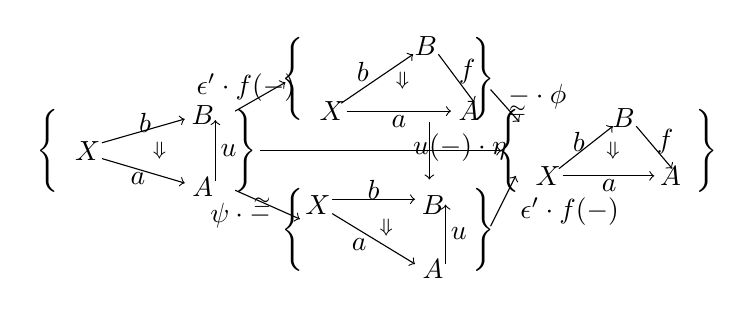
\begin{tikzpicture}[x=1.3em,y=1.3em]
  \begin{scope}[shift={(0,3.2)}]
    \node at (-2.6,0) {$\Bigg\{$};
    \node at (2.9,0) {$\Bigg\}$};
    \node (XL) at (-1.5,0) {$X$};
    \node (BL) at (1.7,1.0) {$B$};
    \node (AL) at (1.7,-1.0) {$A$};
    \draw[->] (-1.1,0.22) -- (1.2,0.88);
    \node at (0.1,0.78) {$b$};
    \draw[->] (-1.1,-0.22) -- (1.2,-0.9);
    \node at (-0.1,-0.78) {$a$};
    \draw[->] (2.05,-0.85) -- (2.05,0.85);
    \node at (2.42,0) {$u$};
    \node at (0.5,0.0) {$\scriptstyle\Downarrow$};
  \end{scope}
  \begin{scope}[shift={(6.4,5.2)}]
    \node at (-2.2,0) {$\Bigg\{$};
    \node at (3.1,0) {$\Bigg\}$};
    \node (XT) at (-1.1,-0.9) {$X$};
    \node (BT) at (1.5,0.9) {$B$};
    \node (AT) at (2.7,-0.9) {$A$};
    \draw[->] (-0.85,-0.68) -- (1.15,0.68);
    \node at (-0.25,0.2) {$b$};
    \draw[->] (1.85,0.68) -- (2.85,-0.66);
    \node at (2.65,0.2) {$f$};
    \draw[->] (-0.7,-0.9) -- (2.2,-0.9);
    \node at (0.75,-1.18) {$a$};
    \node at (0.85,-0.05) {$\scriptstyle\Downarrow$};
  \end{scope}
  \begin{scope}[shift={(6.4,1.0)}]
    \node at (-2.2,0) {$\Bigg\{$};
    \node at (3.1,0) {$\Bigg\}$};
    \node (XB) at (-1.5,0.7) {$X$};
    \node (BB) at (1.7,0.7) {$B$};
    \node (AB) at (1.7,-1.1) {$A$};
    \draw[->] (-1.1,0.85) -- (1.2,0.85);
    \node at (0.05,1.12) {$b$};
    \draw[->] (-1.1,0.45) -- (1.2,-0.95);
    \node at (-0.35,-0.42) {$a$};
    \draw[->] (2.05,-0.95) -- (2.05,0.7);
    \node at (2.42,-0.1) {$u$};
    \node at (0.4,0.05) {$\scriptstyle\Downarrow$};
  \end{scope}
  \begin{scope}[shift={(12.8,3.2)}]
    \node at (-2.6,0) {$\Bigg\{$};
    \node at (2.9,0) {$\Bigg\}$};
    \node (XR) at (-1.5,-0.7) {$X$};
    \node (BR) at (0.6,0.9) {$B$};
    \node (AR) at (1.9,-0.7) {$A$};
    \draw[->] (-1.2,-0.5) -- (0.3,0.68);
    \node at (-0.65,0.25) {$b$};
    \draw[->] (0.95,0.68) -- (1.95,-0.5);
    \node at (1.75,0.25) {$f$};
    \draw[->] (-1.1,-0.7) -- (1.45,-0.7);
    \node at (0.2,-0.98) {$a$};
    \node at (0.3,0.0) {$\scriptstyle\Downarrow$};
  \end{scope}
  \draw[->] (2.6,4.3) -- (4.0,5.1);
  \node at (2.9,4.95) {$\epsilon'\cdot f(-)$};
  \draw[->] (9.7,4.9) -- (10.5,4.0);
  \node at (11.0,4.7) {$-\cdot\phi$};
  \node at (10.45,4.3) {$\scriptstyle\simeq$};
  \draw[->] (2.6,2.1) -- (4.4,1.3);
  \node at (2.75,1.4) {$\psi\cdot-$};
  \node at (3.35,1.75) {$\scriptstyle\simeq$};
  \draw[->] (9.7,1.1) -- (10.4,2.5);
  \node at (11.9,1.5) {$\epsilon'\cdot f(-)$};
  \draw[->] (8.0,4.0) -- (8.0,2.4);
  \node at (8.85,3.3) {$u(-)\cdot\eta$};
  \draw[->] (3.3,3.2) -- (10.0,3.2);
\end{tikzpicture}
\end{center}
由「\trTriangleEqualities{}复合是同构」这一假设，这些函数中有两个可逆，再由\trIsomorphism{}的%
\trTwoOfSixProperty{}，全部六个映射都是双射。
定义「修正过的」\trCounit{}为如下复合：
\begin{center}
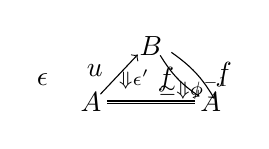
\begin{tikzpicture}[x=1.35em,y=1.35em]
  \node at (-2.9,0.6) {$\epsilon\coloneqq$};
  \node (Bc) at (0,1.5) {$B$};
  \node (A1c) at (-1.6,0) {$A$};
  \node (A2c) at (1.6,0) {$A$};
  \draw[double] (-1.18,0) -- (1.18,0);
  \draw[->] (-1.35,0.22) -- (-0.35,1.28);
  \node at (-1.5,0.85) {$u$};
  \draw[->] (0.25,1.26) to[bend right=12] (1.3,0.16);
  \node at (0.4,0.6) {$f$};
  \draw[->] (0.55,1.34) to[bend left=12] (1.7,0.1);
  \node at (1.95,0.75) {$f$};
  \node at (-0.45,0.62) {$\scriptstyle\Downarrow\epsilon'$};
  \node at (1.15,0.38) {$\scriptstyle\simeq\Downarrow\phi^{-1}$};
\end{tikzpicture}
\end{center}
使得\trTriangleEqualities{}复合之一约化为恒等：
\begin{center}
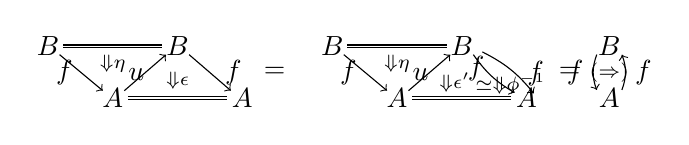
\begin{tikzpicture}[x=1.3em,y=1.25em]
  \node (B1) at (0,1.5) {$B$};
  \node (B2) at (3.6,1.5) {$B$};
  \node (A1) at (1.8,0) {$A$};
  \node (A2) at (5.4,0) {$A$};
  \draw[double] (0.42,1.5) -- (3.18,1.5);
  \draw[double] (2.22,0) -- (4.98,0);
  \draw[->] (0.32,1.26) -- (1.52,0.22);
  \node at (0.45,0.75) {$f$};
  \draw[->] (2.12,0.22) -- (3.28,1.26);
  \node at (2.45,0.68) {$u$};
  \draw[->] (3.92,1.26) -- (5.08,0.22);
  \node at (5.15,0.75) {$f$};
  \node at (1.8,1.0) {$\scriptstyle\Downarrow\eta$};
  \node at (3.6,0.5) {$\scriptstyle\Downarrow\epsilon$};
  \node at (6.3,0.75) {$=$};
  \node (B3) at (7.9,1.5) {$B$};
  \node (B4) at (11.5,1.5) {$B$};
  \node (A3) at (9.7,0) {$A$};
  \node (A4) at (13.3,0) {$A$};
  \draw[double] (8.32,1.5) -- (11.08,1.5);
  \draw[double] (10.12,0) -- (12.88,0);
  \draw[->] (8.22,1.26) -- (9.42,0.22);
  \node at (8.35,0.75) {$f$};
  \draw[->] (10.02,0.22) -- (11.18,1.26);
  \node at (10.35,0.68) {$u$};
  \draw[->] (11.82,1.26) to[bend right=12] (12.97,0.16);
  \node at (11.9,0.85) {$f$};
  \draw[->] (12.07,1.34) to[bend left=12] (13.5,0.14);
  \node at (13.55,0.7) {$f$};
  \node at (9.7,1.0) {$\scriptstyle\Downarrow\eta$};
  \node at (11.3,0.45) {$\scriptstyle\Downarrow\epsilon'$};
  \node at (12.85,0.42) {$\scriptstyle\simeq\Downarrow\phi^{-1}$};
  \node at (14.5,0.75) {$=$};
  \node (Bt) at (15.6,1.5) {$B$};
  \node (At) at (15.6,0) {$A$};
  \draw[->] (15.25,1.26) to[bend right=20] node[left]{$f$} (15.25,0.24);
  \draw[->] (15.95,0.24) to[bend right=20] node[right]{$f$} (15.95,1.26);
  \node at (15.6,0.75) {$\scriptstyle(\Rightarrow)$};
\end{tikzpicture}
\end{center}
现在由粘贴等式
\begin{center}
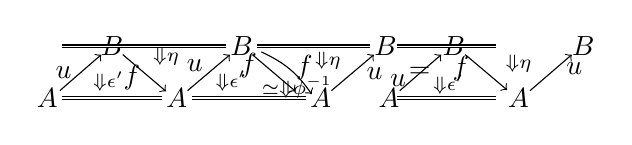
\begin{tikzpicture}[x=1.3em,y=1.25em]
  \node (B1) at (0,1.5) {$B$};
  \node (B2) at (3.6,1.5) {$B$};
  \node (B3) at (7.6,1.5) {$B$};
  \node (A1) at (-1.8,0) {$A$};
  \node (A2) at (1.8,0) {$A$};
  \node (A3) at (5.8,0) {$A$};
  \draw[double] (-1.38,1.5) -- (3.18,1.5);
  \draw[double] (4.02,1.5) -- (7.18,1.5);
  \draw[double] (-1.38,0) -- (1.38,0);
  \draw[double] (2.22,0) -- (5.38,0);
  \draw[->] (-1.45,0.22) -- (-0.3,1.26);
  \node at (-1.35,0.75) {$u$};
  \draw[->] (0.3,1.26) -- (1.5,0.2);
  \node at (0.55,0.6) {$f$};
  \draw[->] (2.1,0.22) -- (3.28,1.26);
  \node at (2.3,0.95) {$u$};
  \draw[->] (3.9,1.26) -- (5.1,0.2);
  \node at (3.8,0.95) {$f$};
  \draw[->] (4.15,1.34) to[bend left=15] (5.55,0.12);
  \node at (5.35,0.9) {$f$};
  \draw[->] (6.1,0.22) -- (7.28,1.26);
  \node at (7.3,0.7) {$u$};
  \node at (-0.1,0.48) {$\scriptstyle\Downarrow\epsilon'$};
  \node at (1.5,1.2) {$\scriptstyle\Downarrow\eta$};
  \node at (3.3,0.5) {$\scriptstyle\Downarrow\epsilon'$};
  \node at (5.14,0.32) {$\scriptstyle\simeq\Downarrow\phi^{-1}$};
  \node at (6.0,1.1) {$\scriptstyle\Downarrow\eta$};
  \node at (8.55,0.75) {$=$};
  \node (B4) at (9.5,1.5) {$B$};
  \node (B5) at (13.1,1.5) {$B$};
  \node (A4) at (7.7,0) {$A$};
  \node (A5) at (11.3,0) {$A$};
  \draw[double] (7.92,1.5) -- (10.68,1.5);
  \draw[double] (7.92,0) -- (10.68,0);
  \draw[->] (8.0,0.22) -- (9.15,1.26);
  \node at (7.95,0.5) {$u$};
  \draw[->] (9.82,1.26) -- (10.98,0.24);
  \node at (9.7,0.85) {$f$};
  \draw[->] (11.62,0.22) -- (12.78,1.26);
  \node at (12.85,0.85) {$u$};
  \node at (9.35,0.4) {$\scriptstyle\Downarrow\epsilon'$};
  \node at (11.3,1.0) {$\scriptstyle\Downarrow\eta$};
\end{tikzpicture}
\end{center}
我们看到 $(u\epsilon\cdot\eta u)\cdot\psi=\psi$。由于 $\psi$ 可逆，可以消去，从而
得出 $u\epsilon\cdot\eta u=\mathrm{id}_u$。
\end{proof}

2-范畴论中有一个标准结果：2-\trCategory{}中的任何\trEquivalence{}都可以被提升为
一个同时还定义\trAdjunction{}的\trEquivalence{}：

\begin{proposition}[\trAdjointEquivalence]\label{prop:adjoint-equivalences}

任何\trEquivalence{}都可以通过修改其中一个 2-\trCell{}而被提升为一个\textbf{\trAdjointEquivalence}
（adjoint equivalence）。也就是说，可以如此选取\trEquivalence{}中的诸可逆
2-\trCell{}，使之满足\trTriangleEqualities{}。因此，若 $f$ 与 $g$ 是互逆的\trEquivalence{}，
则 $f\dashv g$ 且 $g\dashv f$。
\end{proposition}
\begin{proof}
考虑一个由\trFunctor{} $f\colon A\to B$ 与 $g\colon B\to A$ 连同可逆 2-\trCell{}
\begin{center}
\begin{tikzpicture}[x=1.35em,y=1.35em]
  \node (A1) at (0,0) {$A$};
  \node (A2) at (2.6,0) {$A$};
  \draw[double] (0.4,0.14) -- (2.2,0.14);
  \draw[->] (0.4,-0.18) to[bend right=25] node[below]{$gf$} (2.2,-0.18);
  \node at (1.3,-0.15) {$\scriptstyle\simeq\Downarrow\alpha$};   %
  \node at (4.1,0) {及};
  \node (B1) at (5.6,0) {$B$};
  \node (B2) at (8.2,0) {$B$};
  \draw[->] (6.0,0.18) to[bend left=25] node[above]{$fg$} (7.8,0.18);
  \draw[double] (6.0,-0.14) -- (7.8,-0.14);
  \node at (6.9,0.12) {$\scriptstyle\simeq\Downarrow\beta$};   %
\end{tikzpicture}
\end{center}
构成的一个\trEquivalence{}。由于 $\alpha$ 与 $\beta$ 皆可逆，\trTriangleEqualities{}复合亦然，
于是\cref{lem:minimal-adjunction-data}的构造适用。
\end{proof}

\cref{prop:adjoint-equivalences}的一个用途是证明：\trAdjunction{}在\trEquivalence{}%
之下不变：

\begin{proposition}\label{prop:adjunction-equivalence-invariant}
\trInfinityCategory{}之间的\trFunctor{} $u\colon A\to B$ 容许一个\trLeftAdjoint{}，当且仅当
对任意一对等价的\trInfinityCategory{} $A'\simeq A$ 与 $B'\simeq B$，与之等价的%
\trFunctor{} $u'\colon A'\to B'$ 容许一个\trLeftAdjoint{}。
\end{proposition}

我们将会发现，∞-\trCategory{}理论的整体在这种意义下都是\trEquivalence{}不变的。

\begin{proof}
若 $u\colon A\to B$ 容许一个\trLeftAdjoint{}，则把 $f\dashv u$ 与\trAdjointEquivalence
$A'\simeq A$ 及 $B\simeq B'$ 复合，便得到一个与之等价的\trAdjunction{}：
\begin{center}
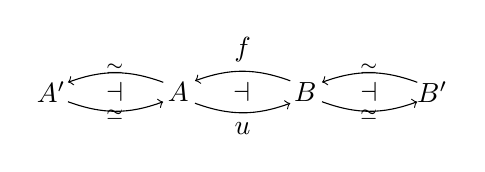
\begin{tikzpicture}[x=1.35em,y=1.35em]
  \node (Ap) at (0,0) {$A'$};
  \node (Am) at (3.4,0) {$A$};
  \node (Bm) at (6.8,0) {$B$};
  \node (Bp) at (10.2,0) {$B'$};
  \draw[->] (3.0,0.26) to[bend right=20] (0.45,0.26);
  \node at (1.7,0.62) {$\scriptstyle\simeq$};
  \node at (1.7,0) {$\dashv$};
  \draw[->] (0.45,-0.26) to[bend right=20] (3.0,-0.26);
  \node at (1.7,-0.62) {$\scriptstyle\simeq$};
  \draw[->] (6.4,0.3) to[bend right=20] node[above]{$f$} (3.85,0.3);
  \node at (5.1,0) {$\dashv$};
  \draw[->] (3.85,-0.3) to[bend right=20] node[below]{$u$} (6.4,-0.3);
  \draw[->] (9.8,0.26) to[bend right=20] (7.25,0.26);
  \node at (8.5,0.62) {$\scriptstyle\simeq$};
  \node at (8.5,0) {$\dashv$};
  \draw[->] (7.25,-0.26) to[bend right=20] (9.8,-0.26);
  \node at (8.5,-0.62) {$\scriptstyle\simeq$};
\end{tikzpicture}
\end{center}
反之，若与之等价的\trFunctor{} $u'\colon A'\simeq A\xrightarrow{\;u\;}B\simeq B'$
容许一个\trLeftAdjoint $f'$，则同样得到一个复合\trAdjunction{}
\begin{center}
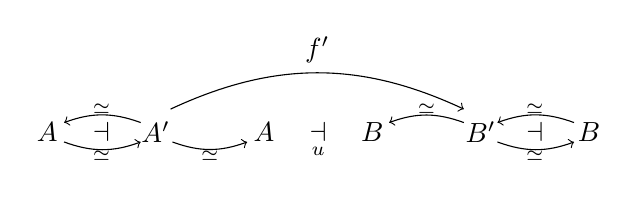
\begin{tikzpicture}[x=1.35em,y=1.35em]
  \node (Al) at (0,0) {$A$};
  \node (Ap) at (2.9,0) {$A'$};
  \node (Am) at (5.8,0) {$A$};
  \node (Bm) at (8.7,0) {$B$};
  \node (Bp) at (11.6,0) {$B'$};
  \node (Br) at (14.5,0) {$B$};
  \draw[->] (2.5,0.26) to[bend right=20] (0.45,0.26);
  \node at (1.45,0.62) {$\scriptstyle\simeq$};
  \node at (1.45,0) {$\dashv$};
  \draw[->] (0.45,-0.26) to[bend right=20] (2.5,-0.26);
  \node at (1.45,-0.62) {$\scriptstyle\simeq$};
  \draw[->] (3.35,-0.26) to[bend right=20] (5.35,-0.26);
  \node at (4.35,-0.62) {$\scriptstyle\simeq$};
  \node at (7.25,0) {$\dashv$};
  \node at (7.25,-0.5) {$\scriptstyle u$};
  \draw[->] (11.15,0.26) to[bend right=20] (9.15,0.26);
  \node at (10.15,0.62) {$\scriptstyle\simeq$};
  \draw[->] (14.1,0.26) to[bend right=20] (12.05,0.26);
  \node at (13.05,0.62) {$\scriptstyle\simeq$};
  \node at (13.05,0) {$\dashv$};
  \draw[->] (12.05,-0.26) to[bend right=20] (14.1,-0.26);
  \node at (13.05,-0.62) {$\scriptstyle\simeq$};
  \draw[->] (3.3,0.62) to[bend left=25] node[above]{$f'$} (11.15,0.62);
\end{tikzpicture}
\end{center}
其\trRightAdjoint{}与原先的\trFunctor{} $u$ 自然同构。于是由\cref{prop:uniqueness-of-adjoints}，
图中所示的\trLeftAdjoint{}就是 $u$ 的一个\trLeftAdjoint{}。
\end{proof}

为备后用，我们以一个抽象定义的\trAdjunction{}作结：经由本节证明的诸结果，它对
任何\trInfinityCosmos{}中的任何\trInfinityCategory{}都能构造出来。

\begin{lemma}\label{lem:composition-adjoint-triple}

对任何\trInfinityCategory{} $A$，「合成」函子
\begin{rveq}\label{eq:composition-functor}
\mbox{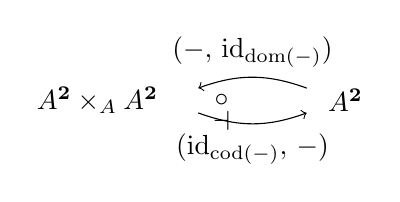
\begin{tikzpicture}[x=1.4em,y=1.4em]
  \node (L) at (0,0) {$A^{\qcTwo}\times_{A}A^{\qcTwo}$};
  \node (R) at (6.4,0) {$A^{\qcTwo}$};
  \draw[->] (5.4,0.32) to[bend right=20] node[above]
    {$(-,\,\mathrm{id}_{\mathrm{dom}(-)})$} (2.6,0.32);
  \node at (3.2,0) {$\circ$};
  \node at (3.2,-0.52) {$\dashv$};
  \draw[->] (2.6,-0.32) to[bend right=20] node[below]
    {$(\mathrm{id}_{\mathrm{cod}(-)},\,-)$} (5.4,-0.32);
\end{tikzpicture}}
\end{rveq}
容许左、右两个伴随，它们把一个箭头延拓成一个可合成的箭头对——分别通过让该箭头
与其定义域处或余域处的恒等箭头配对。
\end{lemma}
\begin{proof}
在 $\Delta\subset\Cat$ 中有一份对偶伴随（dual adjunction）数据，其诸\trFunctor{}%
可用 1.1.1 中引入的单纯算子记号描述：
\begin{center}
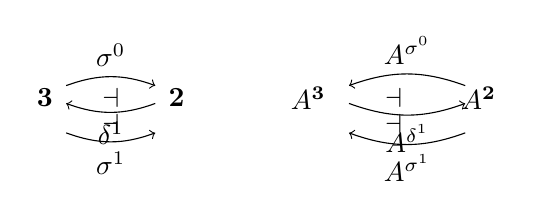
\begin{tikzpicture}[x=1.4em,y=1.4em]
  \node (T1) at (0,0) {$\qcThree$};
  \node (T2) at (3.4,0) {$\qcTwo$};
  \draw[->] (0.55,0.32) to[bend left=20] node[above]{$\sigma^{0}$} (2.85,0.32);
  \node at (1.7,0) {$\dashv$};
  \draw[->] (2.85,-0.14) to[bend left=20] node[below]{$\delta^{1}$} (0.55,-0.14);
  \node at (1.7,-0.66) {$\dashv$};
  \draw[->] (0.55,-0.9) to[bend right=20] node[below]{$\sigma^{1}$} (2.85,-0.9);
  \node at (5.1,0) {$\rightsquigarrow$};
  \node (T3) at (6.8,0) {$A^{\qcThree}$};
  \node (T4) at (11.2,0) {$A^{\qcTwo}$};
  \draw[->] (10.85,0.32) to[bend right=20] node[above]{$A^{\sigma^{0}}$} (7.85,0.32);
  \node at (9.0,0) {$\dashv$};
  \draw[->] (7.85,-0.14) to[bend right=20] node[below]{$A^{\delta^{1}}$} (10.85,-0.14);
  \node at (9.0,-0.66) {$\dashv$};
  \draw[->] (10.85,-0.9) to[bend left=20] node[below]{$A^{\sigma^{1}}$} (7.85,-0.9);
\end{tikzpicture}
\end{center}
对\trInfinityCosmos{} $\mathcal{K}$ 中的任何\trInfinityCategory{} $A$，
\cref{ex:cotensor-2-functor}描述了一个\trTwoFunctor{}
$A^{(-)}\colon\Cat^{op}\to\mathrm{h}\mathcal{K}$，它把上左所示的\trAdjointTriple{}搬运为
上右所示者。

现在我们断言：存在一个平凡\trFibration
$A^{\qcThree}\overset{\sim}{\twoheadrightarrow}A^{\qcTwo}\times_{A}A^{\qcTwo}$，
构造如下。下方左侧的\trSimplicialSet{}\trPushout{}图被单纯\trCotensor{}
$A^{(-)}\colon\sSet^{op}\to\mathcal{K}$ 携带为下方右侧的\trInfinityCategory{}%
\trPullback{}图；由于\trPushout{}方块的诸腿是\trMonomorphism{}，据 1.2.1(ii)，
\trPullback{}方块的诸腿是\trIsofibration{}：
\begin{center}
\begin{tikzpicture}[x=1.5em,y=1.5em]
  \node (PL) at (0,1.4) {$\Lambda^{1}[2]$};
  \node (PT) at (3.2,1.4) {$\qcTwo$};
  \node (PB) at (0,0) {$\qcTwo$};
  \node (PR) at (3.2,0) {$\qcOne$};
  \draw[->] (2.75,1.4) -- (0.75,1.4);
  \draw[->] (0,0.35) -- (0,1.05);
  \draw[->] (3.2,0.35) -- (3.2,1.05);
  \node at (3.62,0.7) {$\delta^{1}$};
  \draw[->] (2.75,0) -- (0.45,0);
  \node at (1.6,-0.34) {$\delta^{0}$};
  \node at (0.42,1.02) {$\scriptstyle\lrcorner$};
  \node at (5.6,0.7) {与};
  \node (QL) at (7.6,1.4) {$A^{\Lambda^{1}[2]}$};
  \node (QT) at (11.6,1.4) {$A^{\qcTwo}$};
  \node (QB) at (7.6,0) {$A^{\qcTwo}$};
  \node (QR) at (11.6,0) {$A$};
  \draw[->] (9.15,1.4) -- (10.25,1.4);
  \draw[->] (7.6,1.05) -- (7.6,0.35);
  \draw[->] (11.6,1.05) -- (11.6,0.35);
  \node at (12.1,0.7) {$\mathrm{ev}_{0}$};
  \draw[->] (9.15,0) -- (10.25,0);
  \node at (10.9,0.34) {$\mathrm{ev}_{1}$};
  \node at (8.02,1.02) {$\scriptstyle\lrcorner$};
\end{tikzpicture}
\end{center}
由引理 1.2.14，内\trHorn{}包含 $\Lambda^{1}[2]\hookrightarrow\Delta[2]\cong\qcThree$
与\trInfinityCategory{} $A$ 的\trCotensor{}定义了一个平凡\trFibration{}
$q\colon A^{\qcThree}\overset{\sim}{\twoheadrightarrow}A^{\Lambda^{1}[2]}\cong A^{\qcTwo}\times_{A}A^{\qcTwo}$。由引理 1.2.18，该平凡\trFibration
$q\colon A^{\qcThree}\overset{\sim}{\twoheadrightarrow}A^{\qcTwo}\times_{A}A^{\qcTwo}$
容许一个\trSection{} $s$，它定义了一个等价逆。由\cref{prop:adjoint-equivalences}，
这些\trFunctor{}既是\trLeftAdjoint{}又是\trRightAdjoint{}。所求的\trAdjointTriple{}便可构造为如下复合%
\trAdjunction{}：
\begin{center}
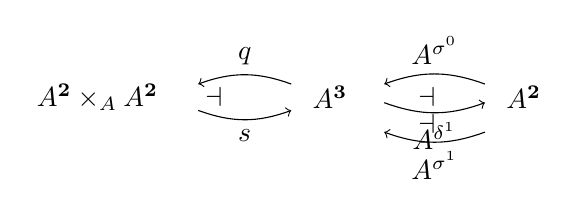
\begin{tikzpicture}[x=1.4em,y=1.4em]
  \node (L) at (0,0) {$A^{\qcTwo}\times_{A}A^{\qcTwo}$};
  \node (M) at (6.0,0) {$A^{\qcThree}$};
  \node (R) at (11.0,0) {$A^{\qcTwo}$};
  \draw[->] (5.0,0.34) to[bend right=20] node[above]{$q$} (2.6,0.34);
  \node at (3.0,0) {$\dashv$};
  \draw[->] (2.6,-0.34) to[bend right=20] node[below]{$s$} (5.0,-0.34);
  \draw[->] (10.0,0.34) to[bend right=20] node[above]{$A^{\sigma^{0}}$} (7.4,0.34);
  \node at (8.5,0) {$\dashv$};
  \draw[->] (7.4,-0.14) to[bend right=20] node[below]{$A^{\delta^{1}}$} (10.0,-0.14);
  \node at (8.5,-0.7) {$\dashv$};
  \draw[->] (10.0,-0.9) to[bend left=20] node[below]{$A^{\sigma^{1}}$} (7.4,-0.9);
\end{tikzpicture}
\end{center}
\end{proof}

注意，\eqref{eq:composition-functor}的诸伴随\trFunctor{}与到 $A\times A$ 的%
\trEndpointEvaluation{}函子可交换。事实上，各\trUnit{}与\trCounit{}同样可以纤维化到 $A\times A$ 之上
（见例 3.6.13）。%

\subsection*{练习}

\begin{exercise}\label{ex:cotensor-2-functor}
本练习的目标是把\cref{rem:contravariant-adjunction-preservation}所讨论的对偶伴随
保持结果中最微妙的一条明确写出来。
\begin{enumerate}[label=(\roman*)]
\item 设 $\mathcal{K}$ 是一个\trInfinityCosmos{}，$A$ 是其中的一个\trInfinityCategory{}。
  证明：单纯\trCotensor{}经限制后定义一个\trTwoFunctor
  $A^{(-)}\colon\mathrm{h}\QCat^{op}\to\mathrm{h}\mathcal{K}$。
\item 论证 (i) 的\trTwoFunctor{}沿\trNerve{}嵌入可进一步限制，从而定义一个%
  \trTwoFunctor{} $A^{(-)}\colon\Cat^{op}\to\mathrm{h}\mathcal{K}$。
\item 结论：对下方左侧所示的 1-\trCategory{}之间的任何\trAdjunction{}，都存在
  右侧所示的\trInfinityCategory{}之间的诱导\trAdjunction{}：
\begin{center}
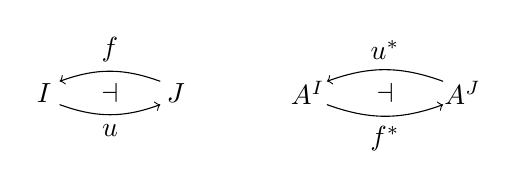
\begin{tikzpicture}[x=1.4em,y=1.4em]
  \node (I) at (0,0) {$I$};
  \node (J) at (3.4,0) {$J$};
  \draw[->] (3.0,0.3) to[bend right=20] node[above]{$f$} (0.4,0.3);
  \node at (1.7,0) {$\dashv$};
  \draw[->] (0.4,-0.3) to[bend right=20] node[below]{$u$} (3.0,-0.3);
  \node at (5.1,0) {$\rightsquigarrow$};
  \node (AI) at (6.8,0) {$A^{I}$};
  \node (AJ) at (10.8,0) {$A^{J}$};
  \draw[->] (10.3,0.3) to[bend right=20] node[above]{$u^{\ast}$} (7.3,0.3);
  \node at (8.8,0) {$\dashv$};
  \draw[->] (7.3,-0.3) to[bend right=20] node[below]{$f^{\ast}$} (10.3,-0.3);
\end{tikzpicture}
\end{center}
\end{enumerate}
\end{exercise}

\begin{exercise}\label{ex:uniqueness-converse}
证明\cref{prop:uniqueness-of-adjoints}(ii)。
\end{exercise}

\begin{exercise}\label{ex:dual-minimal-data}
把\cref{lem:minimal-adjunction-data}的证明对偶化，使之适用于
\cref{prop:adjoint-equivalences}的情形，从而证明：任何\trEquivalence{}都可提升为一个%
\trAdjointEquivalence{}，其中\trCounit{}是原先给定数据的一部分。
\end{exercise}

\begin{exercise}\label{ex:adjoint-equivalence-homotopy-category}
证明：\trInfinityCategory{}之间的\trAdjointEquivalence{}下降为相应\trHomotopyCategory{}之间的%
\trAdjointEquivalence{}。
\end{exercise}
   %
\providecommand{\Fun}{\operatorname{Fun}}
\providecommand{\Cat}{\mathcal{C}at}
\providecommand{\QCat}{\mathcal{Q}\mathcal{C}at}
\providecommand{\qcOne}{\mathbf{1}}   %

\section{\trInitial{}\trElement{}与\trTerminal{}\trElement}\label{sec:initial-and-terminal-elements}

沿用定义 1.4.11 定义\trInfinityCategory{}的\trHomotopyCategory{}时所用的策略，
我们用\trTerminal{}∞-\trCategory{} $1$ 来探查一个\trInfinityCategory{} $A$ 的内部。%
\trHomotopyCategory{} $\mathrm{h}A$ 中的一个对象 $a$，定义为∞-\trCategory{}的映射
$a\colon 1\to A$。为了避免「对象」一词的泛滥，并出于对 Lawvere 的（广义）
\trElement{}概念 \cite{bib74} 的敬意，自此以后我们把映射 $a\colon 1\to A$ 称为%
\trInfinityCategory{} $A$ 的\textbf{\trElement}（element）。\footnote{$A$ 的一个%
\trGeneralizedElement{}是一个\trFunctor{} $f\colon X\to A$。由\trYonedaLemma{}，一个%
\trInfinityCategory{}由其诸\trGeneralizedElement{}决定。}这一术语将帮助我们随时把握
所讨论的「范畴层面」：\trElement $a$ 居于\trInfinityCategory{} $A$ 之中，而后者是%
\trInfinityCosmos{} $\mathcal{K}$ 的对象——这些宇宙本身又定义了「无穷维的范畴」，
尽管属于另一种类型。

\begin{definition}[\trInitial{}\trElement／\trTerminal{}\trElement]\label{def:initial-terminal-element}
\trInfinityCategory{} $A$ 中的一个\textbf{\trInitial{}\trElement}（initial element）是唯一%
\trFunctor{} $!\colon A\to 1$ 的一个\trLeftAdjoint{}，如下左图所示；而%
\trInfinityCategory{} $A$ 中的一个\textbf{\trTerminal{}\trElement}（terminal element）是一个%
\trRightAdjoint{}，如下右图所示。
\begin{center}
\begin{tikzpicture}[x=1.4em,y=1.4em]
  \node (L1) at (0,0) {$1$};
  \node (R1) at (3.6,0) {$A$};
  \draw[->] (0.5,0.32) to[bend left=20] node[above]{$i$} (3.1,0.32);
  \node at (1.8,0) {$\dashv$};
  \draw[->] (3.1,-0.32) to[bend left=20] node[below]{$!$} (0.5,-0.32);
  \node (L2) at (7.2,0) {$1$};
  \node (R2) at (10.8,0) {$A$};
  \draw[->] (10.3,0.32) to[bend right=20] node[above]{$!$} (7.7,0.32);
  \node at (9.0,0) {$\dashv$};
  \draw[->] (7.7,-0.32) to[bend right=20] node[below]{$t$} (10.3,-0.32);
\end{tikzpicture}
\end{center}
\end{definition}

让我们拆解\trInitial{}\trElement{}的定义；对偶的评注适用于\trTerminal{}\trElement{}。

\begin{lemma}[最小数据]\label{lem:minimal-data}
要定义一个\trInfinityCategory{} $A$ 中的\trInitial{}\trElement{}，只须指定：
\begin{itemize}
\item 一个\trElement $i\colon 1\to A$；以及
\item 一个\trNaturalTransformation
\begin{center}
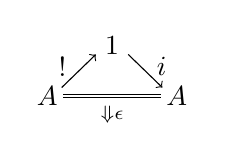
\begin{tikzpicture}[x=1.3em,y=1.3em]
  \node (T) at (1.8,1.4) {$1$};
  \node (L) at (0,0) {$A$};
  \node (R) at (3.6,0) {$A$};
  \draw[->] (0.4,0.24) -- (1.35,1.16);
  \node at (0.42,0.82) {$!$};
  \draw[->] (2.25,1.16) -- (3.2,0.24);
  \node at (3.18,0.82) {$i$};
  \draw[double] (0.45,0) -- (3.15,0);
  \node at (1.8,-0.52) {$\scriptstyle\Downarrow\epsilon$};
\end{tikzpicture}
\end{center}
从常值于 $i$ 的函子到恒同函子，
\end{itemize}
使得其分量 $\epsilon i\colon i\Rightarrow i$——即 $\mathrm{h}A$ 中从 $i$ 到 $i$ 的一个%
箭头——可逆。
\end{lemma}

\begin{proof}
命题 1.4.5——其证明始于该命题陈述之前的一段——表明：\trInfinityCategory{}
$1\in\mathcal{K}$ 在\trHomotopyTwoCategory{} $\mathrm{h}\mathcal{K}$ 中是%
\trTwoTerminalObject{}。这一\trUniversalProperty{}的一维方面蕴含：任何\trElement $i\colon 1\to A$ 都定义了
唯一映射 $!\colon A\to 1$ 的一个\trSection{}；而二维方面则断言：不存在以 $1$ 为
余域的非恒等 2-\trCell{}。特别地，\trAdjunction{} $i\dashv !$ 的\trUnit{}必为恒等，
而\trTriangleEqualities{}之一便自动成立。在此情境下，\cref{def:adjunction}所余的
只是一枚\trCounit{}\trNaturalTransformation{} $\epsilon\colon i!\Rightarrow\mathrm{id}_A$
的数据，连同其分量 $\epsilon i=\mathrm{id}_i$ 这一条件。但事实上，仅从更弱也更
自然的假设——分量 $\epsilon i\colon i\cong i$ 可逆——出发，便可证明这一自然
变换必为恒等。为看清这一点，考虑水平复合
\begin{center}
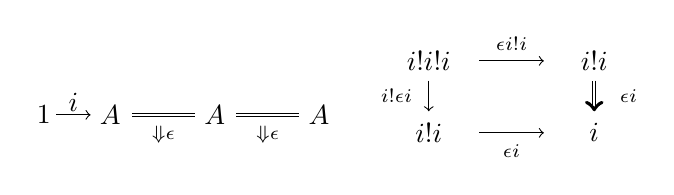
\begin{tikzpicture}[x=1.3em,y=1.3em]
  \node (L1) at (0,0) {$1$};
  \draw[->] (0.35,0) -- (1.3,0);
  \node at (0.82,0.34) {$i$};
  \node (A1) at (1.85,0) {$A$};
  \draw[double] (2.45,0) -- (4.2,0);
  \node at (3.32,-0.55) {$\scriptstyle\Downarrow\epsilon$};
  \node (A2) at (4.75,0) {$A$};
  \draw[double] (5.35,0) -- (7.1,0);
  \node at (6.22,-0.55) {$\scriptstyle\Downarrow\epsilon$};
  \node (A3) at (7.65,0) {$A$};
  \node at (9.15,0) {$\rightsquigarrow$};
  \node (TL) at (10.7,1.5) {$i!i!i$};
  \node (TR) at (15.3,1.5) {$i!i$};
  \node (BL) at (10.7,-0.5) {$i!i$};
  \node (BR) at (15.3,-0.5) {$i$};
  \draw[->] (12.1,1.5) -- (13.9,1.5);
  \node at (13.0,1.98) {$\scriptstyle\epsilon i!i$};
  \draw[->] (10.7,0.95) -- (10.7,0.1);
  \node at (9.8,0.52) {$\scriptstyle i!\epsilon i$};
  \draw[double,->] (15.3,0.95) -- (15.3,0.1);
  \node at (16.25,0.52) {$\scriptstyle\epsilon i$};
  \draw[->] (12.1,-0.5) -- (13.9,-0.5);
  \node at (13.0,-1.0) {$\scriptstyle\epsilon i$};
\end{tikzpicture}
\end{center}
\end{proof}

由\trWhiskering{}的自然性\footnote{「\trWhiskering{}的自然性」（naturality of whiskering）指的是
B.1 节中引理 B.1.3 的观察：2-\trCategory{}中 2-\trCell{}的任何水平复合都可以用
两种不同的方式表达为这些胞腔的若干\trWhiskering{}的竖直复合；在眼下这一情形，它给出了
右上方所展示的 $\mathrm{h}A:=\mathrm{h}\Fun(1,A)$ 中的交换图。
}，我们可以用两种方式把这个复合求值为一个竖直复合。由于 $1$ 是%
\trTwoTerminalObject{}，\trWhiskering{}所得的胞腔 $!\epsilon=\mathrm{id}_!$，于是该复合
关系化归为 $\epsilon i\cdot\epsilon i=\epsilon i$。从而 $\epsilon i$ 是一个
幂等同构，故经消去便是一个恒等。

更简练地说：\trInitial{}\trElement{}定义了\trFunctor{} $!\colon A\twoheadrightarrow 1$ 的一个%
\emph{\trLeftAdjoint{}\trRightInverse}（left adjoint right inverse），而\trTerminal{}\trElement{}定义了一个%
\emph{\trRightAdjoint{}\trRightInverse}（right adjoint right inverse）（见 B.4 节）。

\begin{lemma}[唯一性]\label{lem:uniqueness-of-initial-elements}
\trInfinityCategory{} $A$ 中的任何两个\trInitial{}\trElement{}在 $\mathrm{h}A$ 中同构，而且
$\mathrm{h}A$ 中与某个\trInitial{}\trElement{}同构的任何\trElement{}都是\trInitial{}的。
\end{lemma}
\begin{proof}
由\cref{prop:uniqueness-of-adjoints}，\trFunctor{} $!\colon A\to 1$ 的任何两个%
\trLeftAdjoint{} $i$ 与 $i'$ 自然同构，而任何与 $!\colon A\to 1$ 的一个%
\trLeftAdjoint{}同构的 $a\colon 1\to A$ 本身也是一个\trLeftAdjoint{}。一对\trFunctor{}
$i$ 与 $i'\colon 1\to A$ 之间的\trNaturalTransformation{}同构，恰好给出相应\trElement{}在%
\trHomotopyCategory{} $\mathrm{h}A$ 中的同构 $i\cong i'$ 的数据。
\end{proof}

\begin{remark}\label{rem:representably-initial}
把 2-\trFunctor{} $\Fun(X,-)\colon\mathrm{h}\mathcal{K}\to\mathrm{h}\QCat$ 应用到%
\trInfinityCategory{} $A\in\mathcal{K}$ 的一个\trInitial{}\trElement $i\colon 1\to A$ 上，
便得到一个\trAdjunction
\begin{center}
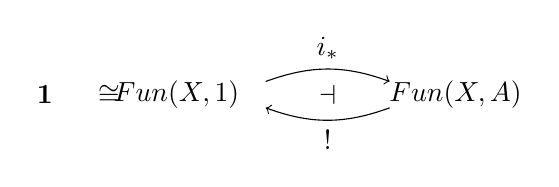
\begin{tikzpicture}[x=1.4em,y=1.4em]
  \node (One) at (0,0) {$\qcOne$};
  \node (F1) at (3.4,0) {$\Fun(X,1)$};
  \node (FA) at (10.6,0) {$\Fun(X,A)$};
  \node at (1.65,0) {$\cong$};
  \draw[->] (5.7,0.34) to[bend left=20] node[above]{$i_{\ast}$} (8.9,0.34);
  \node at (7.3,0) {$\dashv$};
  \draw[->] (8.9,-0.34) to[bend left=20] node[below]{$!$} (5.7,-0.34);
\end{tikzpicture}
\end{center}
经由表达\trTerminal{}∞-\trCategory{} $1$ 之\trUniversalProperty{}的\trIsomorphism{}
$\Fun(X,1)\cong 1$，常值于某个\trInitial{}\trElement{}的\trFunctor
\begin{center}
\begin{tikzpicture}[x=1.4em,y=1.4em]
  \node (X) at (0,0) {$X$};
  \node (One) at (3.4,0) {$1$};
  \node (A) at (6.8,0) {$A$};
  \draw[->] (0.5,0) -- (2.9,0);
  \node at (1.7,0.34) {$!$};
  \draw[->] (3.9,0) -- (6.3,0);
  \node at (5.1,0.34) {$i$};
\end{tikzpicture}
\end{center}
定义了\trFunctorSpace{} $\Fun(X,A)$ 的一个\trInitial{}\trElement{}。这一观察可以概括为：
\trInitial{}\trElement{}在\trInfinityCosmos{}的层面上是\emph{\trRepresentablyInitial}
（representably initial）。

反之，若 $i\colon 1\to A$ 是\trRepresentablyInitial{}，则 $i$ 定义了 $A$ 的一个\trInitial{}\trElement{}。
这一点通过过渡到\trHomotopyTwoCategory{}来看最容易：在其中我们可以证明，一个%
\trInitial{}\trElement $i\colon 1\to A$ 在所有\emph{\trGeneralizedElement}
$f\colon X\to A$ 之中是\trInitial{}的，其确切含义如下。
\end{remark}

\begin{lemma}\label{lem:initial-element-universal-property}
一个\trElement $i\colon 1\to A$ 是\trInitial{}的，当且仅当：对任何 $f\colon X\to A$，
以
\begin{center}
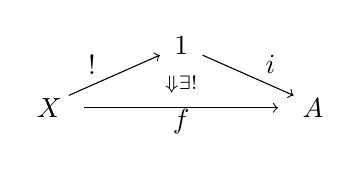
\begin{tikzpicture}[x=1.4em,y=1.4em]
  \node (X) at (0,0) {$X$};
  \node (One) at (3.4,1.6) {$1$};
  \node (A) at (6.8,0) {$A$};
  \draw[->] (0.5,0.32) -- (2.85,1.36);
  \node at (1.1,1.12) {$!$};
  \draw[->] (3.95,1.36) -- (6.3,0.32);
  \node at (5.7,1.12) {$i$};
  \draw[->] (0.9,0) -- (5.9,0);
  \node at (3.4,-0.36) {$f$};
  \node at (3.4,0.6) {$\scriptstyle\Downarrow\exists!$};
\end{tikzpicture}
\end{center}
为边界的 2-\trCell{}存在且唯一。
\end{lemma}

\begin{proof}
若 $i\colon 1\to A$ 是\trInitial{}的，则\cref{def:initial-terminal-element}的%
\trAdjunction{}被 2-\trFunctor{} $\mathrm{h}\Fun(X,-)\colon\mathrm{h}\mathcal{K}\to\Cat$
保持，从而定义了一个\trAdjunction
\begin{center}
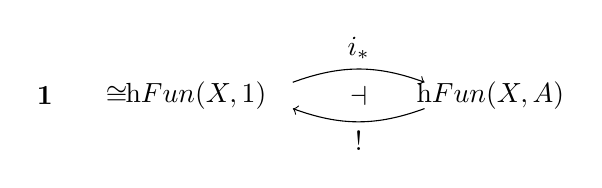
\begin{tikzpicture}[x=1.4em,y=1.4em]
  \node (One) at (0,0) {$\qcOne$};
  \node (F1) at (3.9,0) {$\mathrm{h}\Fun(X,1)$};
  \node (FA) at (11.5,0) {$\mathrm{h}\Fun(X,A)$};
  \node at (1.85,0) {$\cong$};
  \draw[->] (6.4,0.34) to[bend left=20] node[above]{$i_{\ast}$} (9.8,0.34);
  \node at (8.1,0) {$\dashv$};
  \draw[->] (9.8,-0.34) to[bend left=20] node[below]{$!$} (6.4,-0.34);
\end{tikzpicture}
\end{center}
经由\trIsomorphism{} $\mathrm{h}\Fun(X,1)\cong 1$，这个\trAdjunction{}证明了：
\trConstantFunctor{} $i!\colon X\to A$ 在\trCategory{} $\mathrm{h}\Fun(X,A)$ 中是%
\trInitial{}的，从而具有该陈述的\trUniversalProperty{}。

反之，若 $i\colon 1\to A$ 满足该陈述的\trUniversalProperty{}，把它应用于 $A$ 的\trGenericElement{}
（generic element；即恒同映射 $\mathrm{id}_A\colon A\to A$），便产生
\cref{lem:minimal-data}的数据。
\end{proof}

\cref{lem:initial-element-universal-property}说的是：\trInitial{}\trElement{}在%
\trHomotopyTwoCategory{}中是\trRepresentablyInitial{}。把诸\trGeneralizedElement{}特殊化为
通常的\trElement{}，便可见：$A$ 中的\trInitial{}\trElement{}与\trTerminal{}\trElement{}分别定义了其%
\trHomotopyCategory{}中的\trInitial{}\trElement{}与\trTerminal{}\trElement{}：
\begin{rveq}\label{eq:initial-terminal-homotopy-category}
\mbox{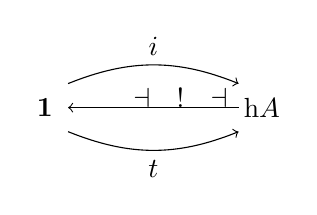
\begin{tikzpicture}[x=1.4em,y=1.4em]
  \node (One) at (0,0) {$\qcOne$};
  \node (hA) at (5.6,0) {$\mathrm{h}A$};
  \draw[->] (0.6,0.62) to[bend left=22] node[above]{$i$} (5.0,0.62);
  \draw[->] (5.0,0) -- (0.6,0);
  \node at (2.5,0.26) {$\dashv$};
  \node at (3.5,0.26) {$!$};
  \node at (4.5,0.26) {$\dashv$};
  \draw[->] (0.6,-0.62) to[bend right=22] node[below]{$t$} (5.0,-0.62);
\end{tikzpicture}}
\end{rveq}

一般而言，「\trHomotopyInitial」（homotopy initial）——即在\trHomotopyCategory{}中%
\trInitial{}——这一性质弱于在\trInfinityCategory{}中\trInitial{}。然而
Nguyen、Raptis 与 Schrade 观察到：\trComplete $(\infty,1)$-\trCategory{}中的一个
同伦\trInitial{}\trElement{}必定定义一个\trInitial{}\trElement \cite[2.2.2]{bib88}。

继续∞-范畴论概念的\trEquivalence{}不变性这一主题：

\begin{lemma}\label{lem:equivalence-invariance-initial-elements}
若 $A$ 有一个\trInitial{}\trElement{}且 $A\simeq A'$，则 $A'$ 有一个\trInitial{}\trElement{}，
并且这些\trElement{}被诸\trEquivalence{}保持至同构。
\end{lemma}
\begin{proof}
由\cref{prop:adjoint-equivalences}，\trEquivalence{} $A\simeq A'$
可以被提升为一个\trAdjointEquivalence{}，而后者立即可与刻画 $A$ 的\trInitial{}\trElement $i$
的那个\trAdjunction{}复合：
\begin{center}
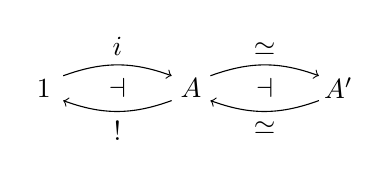
\begin{tikzpicture}[x=1.4em,y=1.4em]
  \node (One) at (0,0) {$1$};
  \node (A) at (3.8,0) {$A$};
  \node (Ap) at (7.6,0) {$A'$};
  \draw[->] (0.5,0.32) to[bend left=20] node[above]{$i$} (3.3,0.32);
  \node at (1.9,0) {$\dashv$};
  \draw[->] (3.3,-0.32) to[bend left=20] node[below]{$!$} (0.5,-0.32);
  \draw[->] (4.3,0.32) to[bend left=20] node[above]{$\simeq$} (7.1,0.32);
  \node at (5.7,0) {$\dashv$};
  \draw[->] (7.1,-0.32) to[bend left=20] node[below]{$\simeq$} (4.3,-0.32);
\end{tikzpicture}
\end{center}
\end{proof}

由\cref{prop:adjunctions-compose}给出的复合\trAdjunction{}证明：$i$ 的像定义了
$A'$ 的一个\trInitial{}\trElement{}，而且由构造，该\trElement{}被\trEquivalence{}
$A\rightsquigarrow A'$ 保持。由\cref{lem:uniqueness-of-initial-elements}所确立的%
\trInitial{}\trElement{}的唯一性，这一论证也表明\trEquivalence{} $A'\rightsquigarrow A$
保持\trInitial{}\trElement{}。

我们现在转向取值于一个\trInfinityCategory{}的\trDiagram{}的\trLimit{}与\trColimit{}的
一般理论。\trInitial{}\trElement{}的理论很好地预演了这一内容：事实上，一个\trInitial{}\trElement
可以被理解为这两个概念各自的实例——\trInitial{}\trElement{}是空图表的\trColimit{}，
同时也是由恒同\trFunctor{}所编码的\trDiagram{}的\trLimit{}，正如我们在\cref{exa:initial-limit-identity}中
所解释的。

\subsection*{练习}

\begin{exercise}\label{ex:representably-initial-element}
用\cref{lem:initial-element-universal-property}证明：如\cref{rem:representably-initial}
所描述的那样，一个可表示地\trInitial{}的\trElement{}必然定义 $A$ 中的一个\trInitial{}\trElement{}。
\end{exercise}

\begin{exercise}\label{ex:preserved-by-adjoints}
证明：\trInitial{}\trElement{}被\trLeftAdjoint{}保持，而\trTerminal{}\trElement{}被%
\trRightAdjoint{}保持。
\end{exercise}
   %
\providecommand{\Fun}{\operatorname{Fun}}
\providecommand{\Cat}{\mathcal{C}at}
\providecommand{\QCat}{\mathcal{Q}\mathcal{C}at}
\providecommand{\sSet}{s\mathcal{S}et}
\providecommand{\qcOne}{\mathbf{1}}   %
\providecommand{\colim}{\operatorname{colim}\nolimits}
\providecommand{\qcTwo}{\mathbf{2}}   %
\providecommand{\CospanShape}{\lrcorner}   %

\section{\trLimit{}与\trColimit}\label{sec:limits-and-colimits}

我们现在来引入在某个\trInfinityCosmos{}中取值于一个\trInfinityCategory{} $A$
\emph{之内}的\trDiagram{}的\trLimit{}与\trColimit{}。我们考虑两种\trDiagram{}：
\begin{itemize}
\item 由单纯集 $J$ 索引、并在一个一般的\trInfinityCosmos{}中取值于一个%
\trInfinityCategory{} $A$ 的\trDiagram{}；以及
\item 由一个\trInfinityCategory{} $J$ 索引、并在一个\trCartesianClosed{}%
\trInfinityCosmos{}中取值于一个\trInfinityCategory{} $A$ 的\trDiagram{}。%
\footnote{对于例 1.2.24 中由 $(\infty,1)$-\trCategory{}构成的那些\trInfinityCosmos{}%
而言，这些概念之间没有本质差别：在 $\QCat$ 中二者同义反复地相同；而在所有与之%
\trBiequivalence{}的\trInfinityCosmos{}中，由\trInfinityCategory{} $J$ 索引%
\trDiagram{}的\trInfinityCategory{}，与把其\trUnderlyingQuasiCategory{}视作一个%
\trSimplicialSet{}来索引\trDiagram{}的\trInfinityCategory{}二者\trEquivalence{}
（见命题 10.3.5）。}
\end{itemize}

\begin{definition}[图表]\label{def:diagram}
所谓\trInfinityCategory{} $A$ 中形状为 $J$ 的一个\textbf{\trDiagram}（diagram），
是指某个\trDiagram{}∞-\trCategory{}的一个\trElement{} $d\colon 1\to A^J$。%
\footnote{当 $A^J$ 是某个\trCartesianClosed{}\trInfinityCosmos{}中的指数时，
\trDiagram{}与\trFunctor{} $d\colon J\to A$ 一一对应。}
这里索引形状 $J$ 或者是一个\trSimplicialSet——此时对包含 $A$ 的任何%
\trInfinityCosmos{} $\mathcal{K}$，$A^J$ 均有定义——或者是一个%
\trInfinityCategory——此时对包含 $A$ 的任何\trCartesianClosed{}%
\trInfinityCosmos{} $\mathcal{K}$，$A^J$ 均有定义。
$J$-索引\trDiagram{}之间的一个态射是\trInfinityCategory{} $A^J$ 中的
一个态射。
\end{definition}

在\trInfinityCosmos{} $\mathcal{K}$ 中构造\trDiagram{}∞-\trCategory{}的两种方式
都定义出\trSimplicial{}双\trFunctor
\begin{equation*}
\sSet^{\mathrm{op}}\times\mathcal{K}\longrightarrow\mathcal{K}
\qquad\qquad
\mathcal{K}^{\mathrm{op}}\times\mathcal{K}\longrightarrow\mathcal{K}
\end{equation*}
\begin{equation*}
(J,A)\longmapsto A^J
\qquad\qquad
(J,A)\longmapsto A^J
\end{equation*}
在两种索引语境中，都存在\trTerminal{}对象 $1$，使得对每个\trInfinityCategory{} $A$
都有 $A^1\cong A$。沿唯一映射 $!\colon J\to 1$ 作限制，便诱导出%
\trConstantFunctor{} $\Delta\colon A\to A^J$。

对于由单纯集索引的\trDiagram{}∞-\trCategory{}与由另一个\trInfinityCategory{}索引的%
\trDiagram{}∞-\trCategory{}，我们有意混用二者的记号，因为我们在第一部分中就前一种
情形证明的所有结果，同样适用于后一种情形。为行文简洁起见，在本节余下部分中我们只
谈及由单纯集索引的\trDiagram{}。

\begin{definition}[\trLimit{}与\trColimit{}函子]\label{def:limit-colimit}
一个\trInfinityCategory{} $A$ \textbf{具备形状 $J$ 的一切\trColimit}（admits all
colimits of shape $J$），如果\trConstantFunctor{} $\Delta\colon A\to A^J$ 容许
一个\trLeftAdjoint{}；而 $A$ \textbf{具备形状 $J$ 的一切\trLimit}（admits all
limits of shape $J$），如果该\trConstantFunctor{}容许一个\trRightAdjoint{}：
\begin{center}
\begin{tikzpicture}[x=1.4em,y=1.4em]
  \node (AJ) at (0,0) {$A^J$};
  \node (A) at (5.4,0) {$A$};
  \draw[->] (1.0,0.66) to[bend left=22] node[above]{$\colim$} (4.4,0.66);
  \node at (2.1,0.30) {$\dashv$};
  \draw[->] (4.4,0) -- (1.0,0);
  \node at (3.4,0.26) {$\Delta$};
  \node at (2.1,-0.30) {$\dashv$};
  \draw[->] (1.0,-0.66) to[bend left=22] node[below]{$\lim$} (4.4,-0.66);
\end{tikzpicture}
\end{center}
在由\trCategory{}组成的\trInfinityCosmos{}中，
\cref{def:limit-colimit}化归为经典定义的\trLimit{}与\trColimit{}函子；
但在一般的\trInfinityCategory{}中，\trLimit{}与\trColimit{}应视作与
经典概念「同伦\trLimit{}」「同伦\trColimit{}」相类比的对象。
在某些情形，这一对应可以精确化：每个\trQuasiCategory{}都%
\trEquivalence{}于某个\trKanComplex\trEnrichedCategory{}的同伦相干\trNerve
\cite[7.2.2]{bib111}，而\trKanComplex\trEnrichedCategory{}中的同伦\trLimit\trCone{}或
同伦\trColimit\trCone{}，恰对应于同伦相干\trNerve{}中的\trLimit\trCone{}或\trColimit\trCone
（见 Lurie 的\cite[4.2.4.1]{bib78}或\cite[6.1.4, 6.2.7]{bib113}）。
在\trInfinityCategory{}的语境中，没有更严格意义的\trLimit{}或%
\trColimit{}概念，所以「同伦」一词通常省去。
\end{definition}

以集合 $J$ 为索引的\trDiagram{}——即索引形状是由集合 $J$ 索引的%
\trTerminal{}对象 $1$ 的\trCoproduct{}的情形——的\trLimit{}或\trColimit{}，
分别称为\trProduct{}或\trCoproduct{}。

\begin{lemma}\label{lem:products-homotopy-category}
\trInfinityCategory{} $A$ 中的\trProduct{}或\trCoproduct{}，也定义出其\trHomotopyCategory{}
$\mathrm{h}A$ 中的\trProduct{}或\trCoproduct{}。
\end{lemma}
\begin{proof}
当 $J$ 是集合时，\trDiagram{}∞-\trCategory{}本身分解为由 $J$ 索引的
$A$ 的副本的\trProduct

\begin{equation*}
A^J\cong\prod_{j\in J}A
\end{equation*}
由于把\trInfinityCategory{}送到其\trHomotopyCategory{}的%
\trTwoFunctor{}
\begin{equation*}
\begin{gathered}
\mathrm{h}\mathcal{K}
\xrightarrow{\ \mathrm{h}\Fun(1,-)\ }\Cat\\
A\longmapsto\mathrm{h}A
\end{gathered}
\end{equation*}
保持\trProduct{}，故当 $J$ 为集合时有 $\mathrm{h}(A^J)\cong\mathrm{h}(\prod_{j\in J}A)\cong\prod_{j\in J}\mathrm{h}A\cong(\mathrm{h}A)^J$。于是，在这一特殊情形，
\cref{def:limit-colimit}中定义\trInfinityCategory{}里的\trProduct{}或\trCoproduct{}的那些%
\trAdjunction{}，便下降为定义其\trHomotopyCategory{}中\trProduct{}或\trCoproduct{}的%
\trAdjunction{}：
\begin{equation*}
\mbox{\begin{tikzpicture}[x=1.4em,y=1.4em]
  \node (hAJ) at (0,0) {$(\mathrm{h}A)^J\cong\mathrm{h}(A^J)$};
  \node (hA) at (7.6,0) {$\mathrm{h}A$};
  \draw[->] (3.3,0.66) to[bend left=22] node[above]{$\colim$} (6.5,0.66);
  \node at (4.4,0.30) {$\dashv$};
  \draw[->] (6.5,0) -- (3.3,0);
  \node at (5.6,0.26) {$\Delta$};
  \node at (4.4,-0.30) {$\dashv$};
  \draw[->] (3.3,-0.66) to[bend left=22] node[below]{$\lim$} (6.5,-0.66);
\end{tikzpicture}}
\end{equation*}
这在 $J=\emptyset$ 的情形依然成立，正解释了\cref{eq:initial-terminal-homotopy-category}中
的观察。
\end{proof}

\begin{warning}\label{war:converse-false}
这一论证并不能推广到更一般的\trLimit{}或\trColimit{}概念，而且%
∞-\trCategory{}中的这类\trLimit{}或\trColimit{}通常并不下降为%
\trHomotopyCategory{}中的\trLimit{}或\trColimit{}。%
\footnote{这类行为在抽象同伦论中是人们熟悉的：同伦\trLimit{}与%
同伦\trColimit{}一般并不是\trHomotopyCategory{}中的\trLimit{}或%
\trColimit{}。}在 §3.2 中，我们将观察到\trHomotopyCategory{}构造%
未能保持更复杂的\trCotensor{}，即便在 $J=\qcTwo$ 这一相对简单的情形中亦然。
\end{warning}

\cref{def:limit-colimit}的问题在于它不够一般：许多\trInfinityCategory{}%
对特定索引形状的\trDiagram{}有某些、但非全部的\trLimit{}。因此，
值得把\cref{def:limit-colimit}重新表述成一种使我们能考虑单个\trDiagram{}
$d\colon 1\to A^J$ 或一族\trDiagram{}之\trLimit{}的形式。为此，
我们利用下面这个 2-\trCategory{}式的概念，它 op-对偶化了更为人熟知的
绝对（\trKanExtension）图。

\begin{definition}[绝对左\trLifting]\label{def:absolute-left-lifting}
在 2-\trCategory{}中给定形如 $C\xrightarrow{g}A\xleftarrow{f}B$ 的图，%
$g$ 沿 $f$ 的一个%
\emph{绝对左\trLifting}（absolute left lifting）由一个 1-\trCell{}
$\ell\colon C\to B$ 及一个 2-\trCell{} $\lambda\colon g\Rightarrow f\ell$
构成，如下左图所示，
使得任何如下中图所示的 2-\trCell{}都能唯一地经由 $(\ell,\lambda)$
分解成如下右图所示的形状：
\begin{center}
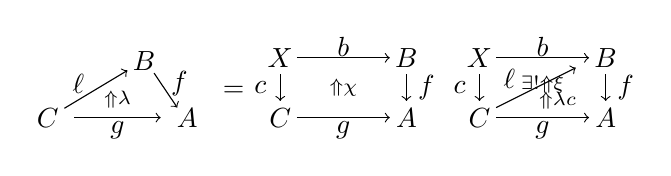
\begin{tikzpicture}[x=1.2em,y=1.2em]
  \node (C1) at (0,0) {$C$};
  \node (A1) at (4.2,0) {$A$};
  \node (B1) at (2.9,1.7) {$B$};
  \draw[->] (0.5,0.28) -- (2.4,1.42);
  \node at (0.92,1.02) {$\ell$};
  \draw[->] (3.2,1.34) -- (3.9,0.3);
  \node at (3.96,1.02) {$f$};
  \draw[->] (0.8,0) -- (3.4,0);
  \node at (2.1,-0.38) {$g$};
  \node at (2.1,0.55) {$\scriptstyle\Uparrow\lambda$};
  \node at (5.6,0.8) {$=$};
  \node (X2) at (7.0,1.8) {$X$};
  \node (B2) at (10.8,1.8) {$B$};
  \node (C2) at (7.0,0) {$C$};
  \node (A2) at (10.8,0) {$A$};
  \draw[->] (7.5,1.8) -- (10.3,1.8);
  \node at (8.9,2.14) {$b$};
  \draw[->] (10.8,1.3) -- (10.8,0.5);
  \node at (11.4,0.9) {$f$};
  \draw[->] (7.0,1.3) -- (7.0,0.5);
  \node at (6.4,0.9) {$c$};
  \draw[->] (7.5,0) -- (10.3,0);
  \node at (8.9,-0.38) {$g$};
  \node at (8.9,0.9) {$\scriptstyle\Uparrow\chi$};
  \node (X3) at (13.0,1.8) {$X$};
  \node (B3) at (16.8,1.8) {$B$};
  \node (C3) at (13.0,0) {$C$};
  \node (A3) at (16.8,0) {$A$};
  \draw[->] (13.5,1.8) -- (16.3,1.8);
  \node at (14.9,2.14) {$b$};
  \draw[->] (16.8,1.3) -- (16.8,0.5);
  \node at (17.4,0.9) {$f$};
  \draw[->] (13.0,1.3) -- (13.0,0.5);
  \node at (12.4,0.9) {$c$};
  \draw[->] (13.5,0) -- (16.3,0);
  \node at (14.9,-0.38) {$g$};
  \draw[->] (13.5,0.3) -- (15.9,1.5);
  \node at (13.9,1.16) {$\ell$};
  \node at (14.9,1.0) {$\scriptstyle\exists!\Uparrow\xi$};
  \node at (15.35,0.5) {$\scriptstyle\Uparrow\lambda c$};
\end{tikzpicture}
\end{center}
对偶地，在 2-\trCategory{}中，$g$ 沿 $f$ 的一个\emph{绝对右\trLifting}（absolute
right lifting）
由一个 1-\trCell{} $r\colon C\to B$ 及一个 2-\trCell{}
$\rho\colon fr\Rightarrow g$ 构成，如下左图所示，
使得任何如下中图所示的 2-\trCell{}都能唯一地经由 $(r,\rho)$
分解成如下右图所示的形状：
\begin{center}
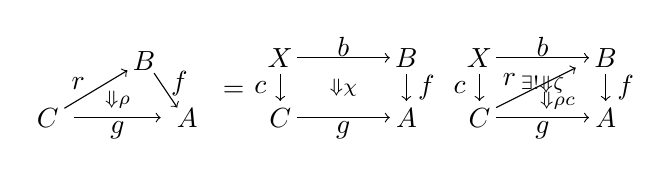
\begin{tikzpicture}[x=1.2em,y=1.2em]
  \node (C1) at (0,0) {$C$};
  \node (A1) at (4.2,0) {$A$};
  \node (B1) at (2.9,1.7) {$B$};
  \draw[->] (0.5,0.28) -- (2.4,1.42);
  \node at (0.92,1.02) {$r$};
  \draw[->] (3.2,1.34) -- (3.9,0.3);
  \node at (3.96,1.02) {$f$};
  \draw[->] (0.8,0) -- (3.4,0);
  \node at (2.1,-0.38) {$g$};
  \node at (2.1,0.55) {$\scriptstyle\Downarrow\rho$};
  \node at (5.6,0.8) {$=$};
  \node (X2) at (7.0,1.8) {$X$};
  \node (B2) at (10.8,1.8) {$B$};
  \node (C2) at (7.0,0) {$C$};
  \node (A2) at (10.8,0) {$A$};
  \draw[->] (7.5,1.8) -- (10.3,1.8);
  \node at (8.9,2.14) {$b$};
  \draw[->] (10.8,1.3) -- (10.8,0.5);
  \node at (11.4,0.9) {$f$};
  \draw[->] (7.0,1.3) -- (7.0,0.5);
  \node at (6.4,0.9) {$c$};
  \draw[->] (7.5,0) -- (10.3,0);
  \node at (8.9,-0.38) {$g$};
  \node at (8.9,0.9) {$\scriptstyle\Downarrow\chi$};
  \node (X3) at (13.0,1.8) {$X$};
  \node (B3) at (16.8,1.8) {$B$};
  \node (C3) at (13.0,0) {$C$};
  \node (A3) at (16.8,0) {$A$};
  \draw[->] (13.5,1.8) -- (16.3,1.8);
  \node at (14.9,2.14) {$b$};
  \draw[->] (16.8,1.3) -- (16.8,0.5);
  \node at (17.4,0.9) {$f$};
  \draw[->] (13.0,1.3) -- (13.0,0.5);
  \node at (12.4,0.9) {$c$};
  \draw[->] (13.5,0) -- (16.3,0);
  \node at (14.9,-0.38) {$g$};
  \draw[->] (13.5,0.3) -- (15.9,1.5);
  \node at (13.9,1.16) {$r$};
  \node at (14.9,1.0) {$\scriptstyle\exists!\Downarrow\zeta$};
  \node at (15.35,0.5) {$\scriptstyle\Downarrow\rho c$};
\end{tikzpicture}
\end{center}
\end{definition}

当这些\trLifting{}存在时，左\trLifting{}与右\trLifting{}分别定义出复合\trFunctor
$f_{\ast}\colon\mathrm{h}\Fun(C,B)\to\mathrm{h}\Fun(C,A)$
的\trLeftAdjoint{}与\trRightAdjoint{}，
而其 2-\trCell{}分别给出这些\trAdjunction{}的\trUnit{}与\trCounit{}%
在对象 $g$ 处的分量。「绝对」这一形容词指的是如下的稳定性。

\begin{lemma}\label{lem:absolute-lifting-restriction}
绝对左\trLifting{}图与绝对右\trLifting{}图在其定义域对象的限制下稳定：
若 $(\ell,\lambda)$ 定义了 $g$ 沿 $f$ 的一个绝对左\trLifting{}，
则对任何 $c\colon X\to C$，限制偶 $(\ell c,\lambda c)$ 定义了
$gc$ 沿 $f$ 的一个绝对左\trLifting{}。
\begin{center}
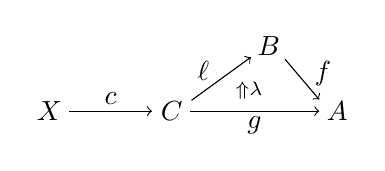
\begin{tikzpicture}[x=1.3em,y=1.3em]
  \node (X) at (0,0) {$X$};
  \node (C) at (3.4,0) {$C$};
  \node (A) at (8.0,0) {$A$};
  \node (B) at (6.1,1.8) {$B$};
  \draw[->] (0.55,0) -- (2.85,0);
  \node at (1.7,0.34) {$c$};
  \draw[->] (3.95,0.3) -- (5.6,1.5);
  \node at (4.28,1.12) {$\ell$};
  \draw[->] (6.55,1.44) -- (7.5,0.32);
  \node at (7.6,1.04) {$f$};
  \draw[->] (3.9,0) -- (7.5,0);
  \node at (5.7,-0.38) {$g$};
  \node at (5.55,0.58) {$\scriptstyle\Uparrow\lambda$};
\end{tikzpicture}
\end{center}
\end{lemma}

\begin{proof}
\cref{lem:absolute-lifting-restriction}的证明是\cref{ex:restriction-absolute-lifting}。
\end{proof}

\trAdjunction{}的\trUnit{}与\trCounit{}分别给出绝对左\trLifting{}图与绝对
右\trLifting{}图的重要例子：

\begin{lemma}\label{lem:unit-counit-absolute-liftings}
一个 2-\trCell{} $\eta\colon\mathrm{id}_B\Rightarrow uf$ 定义某个%
\trAdjunction{} $f\dashv u$ 的\trUnit{}，当且仅当 $(f,\eta)$ 定义一个
绝对左\trLifting{}图：
\begin{center}
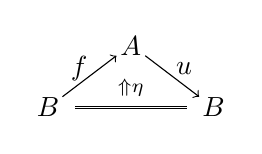
\begin{tikzpicture}[x=1.3em,y=1.3em]
  \node (B1) at (0,0) {$B$};
  \node (B2) at (4.6,0) {$B$};
  \node (T1) at (2.3,1.7) {$A$};
  \draw[->] (0.4,0.3) -- (1.9,1.44);
  \node at (0.86,1.08) {$f$};
  \draw[->] (2.7,1.44) -- (4.2,0.3);
  \node at (3.78,1.08) {$u$};
  \draw[double] (0.75,0) -- (3.85,0);
  \node at (2.3,0.55) {$\scriptstyle\Uparrow\eta$};
\end{tikzpicture}
\end{center}
对偶地，一个 2-\trCell{} $\epsilon\colon fu\Rightarrow\mathrm{id}_A$ 定义
某个\trAdjunction{}的\trCounit{}，当且仅当 $(u,\epsilon)$ 定义一个绝对
右提升图表：
\begin{center}
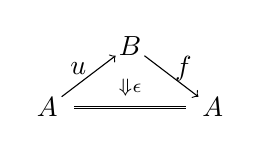
\begin{tikzpicture}[x=1.3em,y=1.3em]
  \node (A1) at (0,0) {$A$};
  \node (A2) at (4.6,0) {$A$};
  \node (T1) at (2.3,1.7) {$B$};
  \draw[->] (0.4,0.3) -- (1.9,1.44);
  \node at (0.86,1.08) {$u$};
  \draw[->] (2.7,1.44) -- (4.2,0.3);
  \node at (3.78,1.08) {$f$};
  \draw[double] (0.75,0) -- (3.85,0);
  \node at (2.3,0.55) {$\scriptstyle\Downarrow\epsilon$};
\end{tikzpicture}
\end{center}
\end{lemma}

\begin{proof}
绝对右\trLifting{}图
\begin{center}
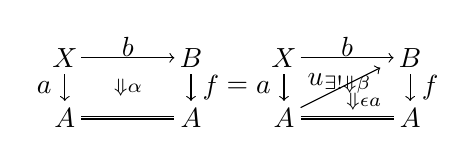
\begin{tikzpicture}[x=1.2em,y=1.2em]
  \node (X1) at (0,1.8) {$X$};
  \node (B1) at (3.8,1.8) {$B$};
  \node (A1) at (0,0) {$A$};
  \node (A2) at (3.8,0) {$A$};
  \draw[->] (0.5,1.8) -- (3.3,1.8);
  \node at (1.9,2.14) {$b$};
  \draw[->] (3.8,1.3) -- (3.8,0.5);
  \node at (4.4,0.9) {$f$};
  \draw[->] (0,1.3) -- (0,0.5);
  \node at (-0.62,0.9) {$a$};
  \draw[double] (0.5,0) -- (3.3,0);
  \node at (1.9,0.9) {$\scriptstyle\Downarrow\alpha$};
  \node at (5.2,0.9) {$=$};
  \node (X2) at (6.6,1.8) {$X$};
  \node (B2) at (10.4,1.8) {$B$};
  \node (A3) at (6.6,0) {$A$};
  \node (A4) at (10.4,0) {$A$};
  \draw[->] (7.1,1.8) -- (9.9,1.8);
  \node at (8.5,2.14) {$b$};
  \draw[->] (10.4,1.3) -- (10.4,0.5);
  \node at (11.0,0.9) {$f$};
  \draw[->] (6.6,1.3) -- (6.6,0.5);
  \node at (5.98,0.9) {$a$};
  \draw[double] (7.1,0) -- (9.9,0);
  \draw[->] (7.1,0.3) -- (9.5,1.5);
  \node at (7.55,1.14) {$u$};
  \node at (8.5,1.0) {$\scriptstyle\exists!\Downarrow\beta$};
  \node at (9.0,0.48) {$\scriptstyle\Downarrow\epsilon a$};
\end{tikzpicture}
\end{center}
的泛性质断言：每个\trNaturalTransformation{}
$\alpha\colon fb\Rightarrow a$ 都有跨同伦 2-\trCategory{}的诸%
\trHomCategory{}之间\trAdjunction{}的唯一转置
$\beta\colon b\Rightarrow ua$：
\begin{center}
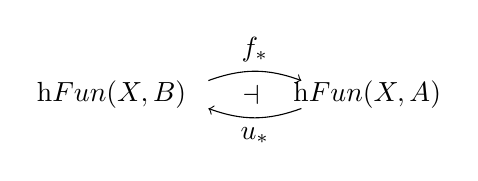
\begin{tikzpicture}[x=1.4em,y=1.4em]
  \node (HB) at (0,0) {$\mathrm{h}\Fun(X,B)$};
  \node (HA) at (6.6,0) {$\mathrm{h}\Fun(X,A)$};
  \draw[->] (2.5,0.36) to[bend left=20] node[above]{$f_{\ast}$} (4.9,0.36);
  \node at (3.6,0) {$\dashv$};
  \draw[->] (4.9,-0.36) to[bend left=20] node[below]{$u_{\ast}$} (2.5,-0.36);
\end{tikzpicture}
\end{center}
于是，若 $f\dashv u$ 带有余单位 $\epsilon$，则\cref{prop:adjunction-preservation}(ii)
便给出这条诱导的\trAdjunction{}，而 $(u,\epsilon)$ 定义 $\mathrm{id}_A$ 沿 $f$
的一个绝对右\trLifting{}。
反过来，一个\trAdjunction{}的\trUnit{}与三角等式可以从绝对右\trLifting{}图的%
\trUniversalProperty{}中提取出来。细节留作\cref{ex:pasting-reproves-unit-counit}。
\end{proof}

特别地，\cref{def:limit-colimit}中\trAdjunction{} $\colim\dashv\Delta\dashv\lim$
的\trUnit{}与\trCounit{}定义出绝对左\trLifting{}图与绝对右\trLifting{}图：
\begin{center}
\begin{tikzpicture}[x=1.3em,y=1.3em]
  \node (AJ1) at (0,0) {$A^{J}$};
  \node (T1) at (2.9,1.7) {$A$};
  \node (AJ2) at (5.8,0) {$A^{J}$};
  \draw[->] (0.45,0.3) -- (2.45,1.42);
  \node at (0.95,1.1) {$\colim$};
  \draw[->] (3.35,1.42) -- (5.35,0.3);
  \node at (4.95,1.1) {$\Delta$};
  \draw[double] (0.75,0) -- (5.05,0);
  \node at (2.9,0.55) {$\scriptstyle\Uparrow\eta$};
  \node at (8.2,0.8) {与};
  \node (AJ3) at (10.6,0) {$A^{J}$};
  \node (T2) at (13.5,1.7) {$A$};
  \node (AJ4) at (16.4,0) {$A^{J}$};
  \draw[->] (11.05,0.3) -- (13.05,1.42);
  \node at (11.62,1.1) {$\lim$};
  \draw[->] (13.95,1.42) -- (15.95,0.3);
  \node at (16.5,1.1) {$\Delta$};
  \draw[double] (11.35,0) -- (15.65,0);
  \node at (13.5,0.55) {$\scriptstyle\Downarrow\epsilon$};
\end{tikzpicture}
\end{center}
由\cref{lem:absolute-lifting-restriction}，这些泛性质在限制到%
\trDiagram{}∞-\trCategory{}的任何\trSubobject{}时依然保持。这激发了如下定义：

\begin{definition}[\trLimit{}与\trColimit]\label{def:limit-colimit-cones}
\trInfinityCategory{} $A$ 中形状为 $J$ 的一族\trDiagram{}
$d\colon D\to A^J$ 的一个\textbf{\trColimit}（colimit）由一个绝对左\trLifting{}图
\begin{center}
\begin{tikzpicture}[x=1.3em,y=1.3em]
  \node (D) at (0,0) {$D$};
  \node (T) at (2.9,1.7) {$A$};
  \node (R) at (5.8,0) {$A^J$};
  \draw[->] (0.45,0.3) -- (2.45,1.42);
  \node at (0.95,1.1) {$\colim d$};
  \draw[->] (3.35,1.42) -- (5.35,0.3);
  \node at (4.9,1.1) {$\Delta$};
  \draw[->] (0.75,0) -- (5.05,0);
  \node at (2.9,-0.38) {$d$};
  \node at (2.9,0.55) {$\scriptstyle\Uparrow\eta$};
\end{tikzpicture}
\end{center}
给出，它由一个\trGeneralizedElement{} $\colim d\colon D\to A$ 连同一个%
\trColimit\trCone $\eta\colon d\Rightarrow\Delta\colim d$ 构成。

对偶地，\trInfinityCategory{} $A$ 中形状为 $J$ 的一族\trDiagram{}
$d\colon D\to A^J$ 的一个\textbf{\trLimit}（limit）由一个绝对右\trLifting{}图
\begin{center}
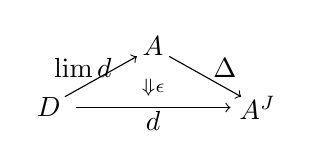
\begin{tikzpicture}[x=1.3em,y=1.3em]
  \node (D) at (0,0) {$D$};
  \node (T) at (2.9,1.7) {$A$};
  \node (R) at (5.8,0) {$A^J$};
  \draw[->] (0.45,0.3) -- (2.45,1.42);
  \node at (0.95,1.1) {$\lim d$};
  \draw[->] (3.35,1.42) -- (5.35,0.3);
  \node at (4.9,1.1) {$\Delta$};
  \draw[->] (0.75,0) -- (5.05,0);
  \node at (2.9,-0.38) {$d$};
  \node at (2.9,0.55) {$\scriptstyle\Downarrow\epsilon$};
\end{tikzpicture}
\end{center}
给出，它由一个\trGeneralizedElement{} $\lim d\colon D\to A$ 连同一个%
\trLimit\trCone $\epsilon\colon\Delta\lim d\Rightarrow d$ 构成。
\end{definition}

\begin{remark}\label{rem:families-of-diagrams}
若 $A$ 具有 $J$ 形状的所有\trLimit{}，则\cref{lem:absolute-lifting-restriction}
蕴含：任何\trDiagram{}族 $d\colon D\to A^J$ 都有\trLimit{}，它由把\trLimit{}%
函子 $\lim\colon A^J\to A$ 与 $d$ 复合而定义。在一个由 $(\infty,1)$-\trCategory{}%
构成的\trInfinityCosmos{}中，若每个\trDiagram{} $d\colon 1\to A^J$ 都有%
\trLimit{}，则 $A$ 具有 $J$ 形状的所有\trLimit{}（见推论 12.2.10）；
但在一般情形，\trDiagram{}族无法化归为单个\trDiagram{}。
\end{remark}

\begin{example}[\trInitial{}\trElement{}是\trEmptyDiagram{}的\trColimit]%
\label{exa:initial-colimit-empty}
一个\trInitial{}\trElement{}定义任意\trInfinityCategory{} $A$ 中形状
$\emptyset$ 的\trEmptyDiagram{}的一个\trColimit{}。由 $A$ 中空图表构成的%
\trInfinityCategory{} $A^{\emptyset}\simeq\qcOne$ 是\trTerminal{}的，%
故\trConstantFunctor{}化为 $!\colon A\to 1$。
要证明\trInitial{}\trElement{}是\cref{def:limit-colimit-cones}意义上的%
\trColimit{}，我们必须验证：一个\trInitial{}\trElement{}定义一个%
2-\trCell{}为恒同的绝对左\trLifting{}图
\begin{center}
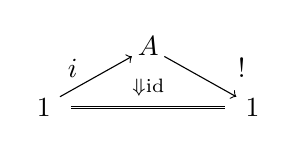
\begin{tikzpicture}[x=1.3em,y=1.3em]
  \node (One) at (0,0) {$1$};
  \node (A) at (2.9,1.7) {$A$};
  \node (OneR) at (5.8,0) {$1$};
  \draw[->] (0.45,0.3) -- (2.45,1.42);
  \node at (0.8,1.1) {$i$};
  \draw[->] (3.35,1.42) -- (5.35,0.3);
  \node at (5.5,1.1) {$!$};
  \draw[double] (0.75,0) -- (5.05,0);
  \node at (2.9,0.55) {$\scriptstyle\Downarrow\mathrm{id}$};
\end{tikzpicture}
\end{center}
\begin{center}
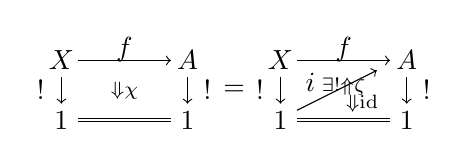
\begin{tikzpicture}[x=1.2em,y=1.2em]
  \node (X1) at (0,1.8) {$X$};
  \node (A1) at (3.8,1.8) {$A$};
  \node (O1) at (0,0) {$1$};
  \node (O2) at (3.8,0) {$1$};
  \draw[->] (0.5,1.8) -- (3.3,1.8);
  \node at (1.9,2.14) {$f$};
  \draw[->] (3.8,1.3) -- (3.8,0.5);
  \node at (4.4,0.9) {$!$};
  \draw[->] (0,1.3) -- (0,0.5);
  \node at (-0.62,0.9) {$!$};
  \draw[double] (0.5,0) -- (3.3,0);
  \node at (1.9,0.9) {$\scriptstyle\Downarrow\chi$};
  \node at (5.2,0.9) {$=$};
  \node (X2) at (6.6,1.8) {$X$};
  \node (A2) at (10.4,1.8) {$A$};
  \node (O3) at (6.6,0) {$1$};
  \node (O4) at (10.4,0) {$1$};
  \draw[->] (7.1,1.8) -- (9.9,1.8);
  \node at (8.5,2.14) {$f$};
  \draw[->] (10.4,1.3) -- (10.4,0.5);
  \node at (11.0,0.9) {$!$};
  \draw[->] (6.6,1.3) -- (6.6,0.5);
  \node at (5.98,0.9) {$!$};
  \draw[double] (7.1,0) -- (9.9,0);
  \draw[->] (7.1,0.3) -- (9.5,1.5);
  \node at (7.5,1.14) {$i$};
  \node at (8.5,1.0) {$\scriptstyle\exists!\Uparrow\zeta$};
  \node at (9.05,0.5) {$\scriptstyle\Downarrow\mathrm{id}$};
\end{tikzpicture}
\end{center}
由于∞-\trCategory{} $1$ 是\trTwoTerminalObject{}，居于上面方图中的
2-\trCell{} $\chi$ 是唯一的，即恒同。于是，该绝对左\trLifting{}图的泛性质
断言：对任何 $f\colon X\to A$，存在唯一的 2-\trCell{}
$\zeta\colon i!\Rightarrow f$——恰如\cref{lem:initial-element-universal-property}
所给出者。
\end{example}

\begin{example}[\trInitial{}\trElement{}是恒同\trFunctor{}的\trLimit]%
\label{exa:initial-limit-identity}
在\trCartesianClosed{}\trInfinityCosmos{}中，\trInitial{}\trElement{}
$i\colon 1\to A$ 还可以看作恒同\trFunctor{} $\mathrm{id}_A\colon A\to A$
的一个\trLimit{}。\footnote{这一结果在命题 9.4.10 中推广到非\trCartesianClosed{}
\trInfinityCosmos{}。%
}\trAdjunction{} $i\dashv !$ 的\trCounit{}
$\epsilon\colon i!\Rightarrow\mathrm{id}_A$ 跨命题 1.4.5 的 2-\trAdjunction{}
$A\times-\dashv(-)^{A}$ 转置，定义出下左图所示的\trLimit\trCone
\begin{center}
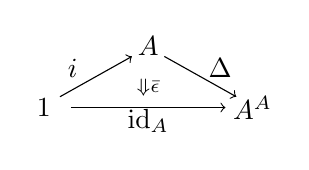
\begin{tikzpicture}[x=1.3em,y=1.3em]
  \node (One) at (0,0) {$1$};
  \node (A) at (2.9,1.7) {$A$};
  \node (AA) at (5.8,0) {$A^{A}$};
  \draw[->] (0.45,0.3) -- (2.45,1.42);
  \node at (0.8,1.1) {$i$};
  \draw[->] (3.35,1.42) -- (5.35,0.3);
  \node at (4.9,1.1) {$\Delta$};
  \draw[->] (0.75,0) -- (5.05,0);
  \node at (2.9,-0.38) {$\mathrm{id}_A$};
  \node at (2.9,0.55) {$\scriptstyle\Downarrow\bar\epsilon$};
\end{tikzpicture}
\end{center}
其绝对性（从而其泛性质）可验证如下。对任何 $f\colon X\to A$，须证每个
2-\trCell{} $\chi\colon\Delta f\Rightarrow(\mathrm{id}_A)!$——即以 $f$
为顶点、覆盖该\trDiagram{}的一个\trCone——都通过唯一的
$\zeta\colon f\Rightarrow i!$ 而分解：
\begin{center}
\begin{tikzpicture}[x=1.15em,y=1.15em]
  \node (X1) at (0,1.9) {$X$};
  \node (A1) at (4.2,1.9) {$A$};
  \node (O1) at (0,0) {$1$};
  \node (AA1) at (4.2,0) {$A^{A}$};
  \draw[->] (0.55,1.9) -- (3.65,1.9);
  \node at (2.1,2.24) {$f$};
  \draw[->] (4.2,1.4) -- (4.2,0.5);
  \node at (4.85,0.95) {$\Delta$};
  \draw[->] (0,1.4) -- (0,0.5);
  \node at (-0.66,0.95) {$!$};
  \draw[->] (0.55,0) -- (3.65,0);
  \node at (2.1,-0.4) {$\mathrm{id}_A$};
  \node at (2.1,0.95) {$\scriptstyle\Downarrow\chi$};
  \node at (5.9,0.95) {$=$};
  \node (X2) at (7.4,1.9) {$X$};
  \node (A2) at (11.6,1.9) {$A$};
  \node (O2) at (7.4,0) {$1$};
  \node (AA2) at (11.6,0) {$A^{A}$};
  \draw[->] (7.95,1.9) -- (11.05,1.9);
  \node at (9.5,2.24) {$f$};
  \draw[->] (11.6,1.4) -- (11.6,0.5);
  \node at (12.25,0.95) {$\Delta$};
  \draw[->] (7.4,1.4) -- (7.4,0.5);
  \node at (6.74,0.95) {$!$};
  \draw[->] (7.95,0) -- (11.05,0);
  \node at (9.5,-0.4) {$\mathrm{id}_A$};
  \draw[->] (7.95,0.3) -- (10.65,1.6);
  \node at (8.35,1.2) {$i$};
  \node at (9.5,1.05) {$\scriptstyle\exists!\Downarrow\zeta$};
  \node at (10.15,0.45) {$\scriptstyle\Downarrow\bar\epsilon$};
\end{tikzpicture}
\end{center}
这一泛性质最容易通过再次跨 2-\trAdjunction{} $A\times-\dashv(-)^{A}$
转置来验证\yizhu{$\hat\chi$ 恒指 $\chi$ 的转置。}；此时我们必须建立
粘贴等式
\begin{rveq}\label{eq:ex2311-pasting}
\mbox{\begin{tikzpicture}[x=1.15em,y=1.15em]
  \node (XA1) at (0,0.9) {$X\times A$};
  \node (X1) at (3.3,2.3) {$X$};
  \node (A1) at (5.1,0) {$A$};
  \draw[->] (1.1,1.4) -- (2.75,2.1);
  \node at (1.4,2.0) {$\pi_X$};
  \draw[->] (3.75,2.0) -- (4.85,0.45);
  \node at (4.5,1.4) {$f$};
  \draw[->] (1.15,0.6) -- (4.55,0.1);
  \node at (2.8,0.66) {$\pi_A$};
  \node at (3.0,1.2) {$\scriptstyle\Downarrow\hat\chi$};
  \node at (6.6,1.15) {$=$};
  \node (XA2) at (8.0,0.9) {$X\times A$};
  \node (X2) at (11.1,2.3) {$X$};
  \node (One) at (13.2,0.9) {$1$};
  \node (A2) at (16.2,0.9) {$A$};
  \draw[->] (9.1,1.4) -- (10.6,2.1);
  \node at (9.4,2.0) {$\pi_X$};
  \draw[->] (11.6,2.15) to[bend left=20] (16.1,1.4);
  \node at (14.2,2.55) {$f$};
  \draw[->] (11.5,2.0) -- (12.8,1.25);
  \node at (11.85,1.45) {$!$};
  \draw[->] (13.7,0.9) -- (15.6,0.9);
  \node at (14.65,1.18) {$i$};
  \draw[->] (9.15,0.4) -- (15.85,0.62);
  \node at (12.4,-0.05) {$\pi_A$};
  \node at (12.7,1.6) {$\scriptstyle\exists!\Downarrow\zeta$};
  \node at (15.0,0.28) {$\scriptstyle\Downarrow\bar\epsilon$};
  \draw[double] (16.9,0.9) -- (17.8,0.9);
\end{tikzpicture}}
\end{rveq}
注意，把\cref{eq:ex2311-pasting}的右端沿函子
$\mathrm{id}_X\times i\colon X\cong X\times 1\to X\times A$ 限制，就回收了
2-\trCell{} $\zeta$，因为 $\bar\epsilon i=\mathrm{id}_i$。这告诉我们：
给定 $\chi$，我们必须把 2-\trCell{} $\zeta\colon f\Rightarrow i!$ 定义为
$\hat\chi$ 沿函子 $\mathrm{id}_X\times i\colon X\to X\times A$ 的限制。
由 $\zeta$ 的这一定义与笛卡尔积的 \trTwoFunctor{}性——它告诉我们
$\epsilon\pi_A=\pi_A(X\times\epsilon)$——可得
\begin{center}
\begin{tikzpicture}[x=1.2em,y=1.2em]
  \node (X1) at (0,1.8) {$X$};
  \node (A1) at (4.4,1.8) {$A$};
  \node (O1) at (2.2,0.85) {$1$};
  \node (XA1) at (0,0) {$X\times A$};
  \node (A2) at (4.4,0) {$A$};
  \draw[->] (0.55,2.0) to[bend left=22] (3.85,2.0);
  \node at (2.2,2.52) {$f$};
  \draw[->] (0,1.3) -- (0,0.5);
  \node at (-0.66,0.9) {$\pi_X$};
  \draw[->] (0.5,1.5) -- (1.8,1.08);
  \node at (0.9,1.46) {$!$};
  \draw[->] (2.62,1.0) -- (3.9,1.55);
  \node at (3.45,1.02) {$i$};
  \draw[->] (0.55,0) -- (3.85,0);
  \node at (2.2,-0.4) {$\pi_A$};
  \node at (1.3,1.62) {$\scriptstyle\exists!\Downarrow\zeta$};
  \node at (3.4,0.42) {$\scriptstyle\Downarrow\bar\epsilon$};
  \draw[double] (5.0,1.8) -- (5.9,1.8);
  \node at (6.0,0.9) {$=$};
  \node (XA3) at (7.4,0) {$X\times A$};
  \node (XO) at (9.9,1.8) {$X\times 1$};
  \node (XA4) at (12.4,0) {$X\times A$};
  \node (X2) at (16.2,1.8) {$X$};
  \node (A3) at (16.2,0) {$A$};
  \draw[double] (8.5,0) -- (11.3,0);
  \draw[->] (7.95,0.32) -- (9.2,1.42);
  \node at (7.7,1.22) {$\mathrm{id}_X\times !$};
  \draw[->] (10.65,1.42) -- (11.9,0.32);
  \node at (11.65,1.22) {$\mathrm{id}_X\times i$};
  \node at (9.9,0.72) {$\scriptstyle\Downarrow X\times\epsilon$};
  \draw[->] (13.1,0.32) -- (15.7,1.5);
  \node at (14.1,1.2) {$\pi_X$};
  \draw[->] (16.2,1.3) -- (16.2,0.5);
  \node at (16.82,0.9) {$f$};
  \draw[->] (13.1,0) -- (15.7,0);
  \node at (14.4,-0.4) {$\pi_A$};
  \node at (14.75,0.62) {$\scriptstyle\Downarrow\hat\chi$};
\end{tikzpicture}
\end{center}
由「\trWhiskering{}的自然性」（见附录 B 中的\cref{lem:naturality-of-whiskering}），右端的粘贴复合可以求值为
$\pi_X(X\times\epsilon)$ 继以 $\hat\chi$ 的竖直复合，而
$\pi_X(X\times\epsilon)$ 是恒同 2-\trCell{}，故该复合就是 $\hat\chi$。
这就验证了所要的粘贴等式\cref{eq:ex2311-pasting}。
\end{example}

∞-\trCategory{}中的某些\trLimit{}与\trColimit{}因形式上的理由而存在。例如，
一条抽象的 2-\trCategory{}式引理使得同伦论中的一项经典结果得以有一个
形式化的证明，该结果计算「可裂」\trSimplicialObject{}的诸\trColimit{}，
这些\trColimit{}通常称作\trGeometricRealization{}。在证明这一点之前，
我们先引入所涉及的索引形状。

\begin{definition}[\trSplit{}\trAugmented{}（余）\trSimplicialObject]\label{def:split-augmented}
在定义 1.1.1 中引入的、由有限非空序数与保序映射组成的\trSimplexCategory{}
$\Delta$，构成由有限序数与保序映射组成的\trCategory{} $\Delta_{+}$ 的
全子范畴，
后者自由地添入空序数 $[-1]$ 作为\trInitial{}对象。\trCategory{} $\Delta_{+}$
又构成\trCategory{}
$\Delta_{\perp}$ 的宽子范畴，后者在每一对相邻序数之间添入一枚「额外的」
\trDegeneracyOperator{} $\sigma^{-1}\colon[n+1]\twoheadrightarrow[n]$，包括
$\sigma^{-1}\colon[0]\twoheadrightarrow[-1]$。\trCategory{} $\Delta_{+}$ 还构成\trCategory{}
$\Delta_{\top}$
的宽子范畴，后者在每一对相邻序数之间于另一侧添入一枚「额外的」
\trDegeneracyOperator{} $\sigma^{n+1}\colon[n+1]\twoheadrightarrow[n]$，包括 $\sigma^{0}\colon[0]\twoheadrightarrow[-1]$。
范畴 $\Delta_{\perp}$ 与 $\Delta_{\top}$ 还可以按另一种方式来描述：存在从它们到
$\Delta$ 中的忠实嵌入，其在对象上的作用为 $[n]\mapsto[n+1]$，并把 $\Delta_{\perp}$
与 $\Delta_{\top}$ 分别等同于有限非空序数与保序映射中保持底元素或保持顶元素者
所构成的子范畴。以 $\Delta\subset\Delta_{+}\subset\Delta_{\perp},\Delta_{\top}$
为索引的共变\trDiagram{}分别称为\textbf{\trCosimplicialObject}（cosimplicial
objects）、\textbf{余增广\trCosimplicialObject}（coaugmented cosimplicial
objects）与\textbf{\trSplit{}余增广\trCosimplicialObject}（split coaugmented
cosimplicial objects）（无论对 $\Delta_{\perp}$ 还是对 $\Delta_{\top}$ 而言）；
而反变\trDiagram{}则分别称为\textbf{\trSimplicialObject}（simplicial objects）、%
\textbf{\trAugmented{}\trSimplicialObject}（augmented simplicial objects）与%
\textbf{\trSplit{}\trAugmented{}\trSimplicialObject}（split augmented simplicial
objects）。当需要消歧 $\Delta_{\perp}$ 与 $\Delta_{\top}$ 时，我们把前一个范畴
称作一种「底部可裂」（bottom splitting），把后一个范畴称作一种「顶部可裂」
（top splitting），但这一术语并非标准。

\trInfinityCategory{} $A$ 中的一个\trCosimplicialObject{} $d\colon 1\to A^{\Delta}$
\textbf{容许一个余增广}（admits a coaugmentation）或\textbf{容许一个裂分}（admits
a splitting），如果它沿诸限制\trFunctor{}提升
\begin{center}
\begin{tikzpicture}[x=1.3em,y=1.3em]
  \node (Atop) at (3.4,3.4) {$A^{\Delta_{\perp}}$};
  \node (Amid) at (3.4,1.7) {$A^{\Delta_{+}}$};
  \node (Abot) at (3.4,0) {$A^{\Delta}$};
  \node (One) at (0,0) {$1$};
  \draw[->] (3.4,2.9) -- (3.4,2.3);
  \node at (4.5,2.6) {$\mathrm{res}$};
  \draw[->] (3.4,1.2) -- (3.4,0.6);
  \node at (4.5,0.9) {$\mathrm{res}$};
  \draw[->] (0.5,0) -- (2.25,0);
  \node at (1.35,-0.42) {$d$};
  \draw[->,dashed] (0.55,0.3) -- (2.65,1.5);
  \draw[->,dotted] (0.45,0.44) -- (2.8,3.15);
\end{tikzpicture}
\end{center}
而在顶部可裂的情形中，$\Delta_{\perp}$ 被替换为 $\Delta_{\top}$。容许余增广与
裂分的\trCosimplicialObject{}之族，由\trGeneralizedElement{}
$\mathrm{res}\colon A^{\Delta_{\perp}}\twoheadrightarrow A^{\Delta}$ 展示。
\end{definition}

在任何\trAugmented{}\trCosimplicialObject{}中，其底\trCosimplicialObject{}上都存在
一个\trCone{}，其顶点由在 $[-1]\in\Delta_{+}$ 处取值而得。这个\trCone{}由把
唯一的\trNaturalTransformation{}
\begin{rveq}\label{eq:nu-initial-transformation}
\mbox{\begin{tikzpicture}[x=1.3em,y=1.3em]
  \node (D) at (0,0) {$\Delta$};
  \node (Dp) at (5.2,0) {$\Delta_{+}$};
  \node (One) at (2.6,-1.9) {$\qcOne$};
  \draw[->] (0.7,0.15) -- (4.5,0.15);
  \node at (2.6,0.49) {$\scriptstyle\subseteq$};
  \draw[->] (0.6,-0.4) -- (2.1,-1.6);
  \node at (0.98,-1.2) {$!$};
  \draw[->] (3.1,-1.6) -- (4.6,-0.4);
  \node at (4.25,-1.2) {$[-1]$};
  \node at (2.6,-0.75) {$\scriptstyle\Uparrow\exists!\nu$};
\end{tikzpicture}}
\end{rveq}
与 $A$ 作余张量而定义；这一\trNaturalTransformation{}之所以存在，是因为
$[-1]\colon\qcOne\to\Delta_{+}$ 是\trInitial{}对象（见\cref{lem:initial-element-universal-property}）。

\begin{proposition}[\trTotalization{}/\trGeometricRealization]\label{prop:split-limits}
设 $A$ 为任一\trInfinityCategory{}。$A$ 中每个容许余增广与裂分的%
\trCosimplicialObject{}都有一个\trLimit{}，其\trLimit\trCone{}由余增广定义；
对偶地，$A$ 中每个容许增广与裂分的\trSimplicialObject{}都有一个%
\trColimit{}，其\trColimit\trCone{}由增广定义。也就是说，存在绝对的
右\trLifting{}图与左\trLifting{}图
\begin{center}
\begin{tikzpicture}[x=1.0em,y=1.0em]
  \node (B1) at (0,0) {$A^{\Delta_{\perp}}$};
  \node (T1) at (4.2,2.2) {$A^{\Delta_{+}}$};
  \node (T1R) at (8.4,2.2) {$A$};
  \node (R1) at (8.4,0) {$A^{\Delta}$};
  \draw[->] (1.9,0.35) -- (3.25,1.5);
  \node at (1.9,1.25) {$\mathrm{res}$};
  \draw[->] (5.5,2.2) -- (7.3,2.2);
  \node at (6.4,2.54) {$\mathrm{ev}_{[-1]}$};
  \draw[->] (8.4,1.6) -- (8.4,0.55);
  \node at (9.15,1.05) {$\Delta$};
  \draw[->] (1.9,0) -- (7.4,0);
  \node at (4.65,-0.38) {$\mathrm{res}$};
  \node at (4.9,1.0) {$\scriptstyle\Downarrow A^{\nu}$};
  \node (B2) at (13.5,0) {$A^{(\Delta_{\perp})^{\mathrm{op}}}$};
  \node (T2) at (18.5,2.2) {$A^{(\Delta_{+})^{\mathrm{op}}}$};
  \node (T2R) at (23.5,2.2) {$A$};
  \node (R2) at (23.5,0) {$A^{\Delta^{\mathrm{op}}}$};
  \draw[->] (16.1,0.35) -- (17.25,1.5);
  \node at (16.1,1.25) {$\mathrm{res}$};
  \draw[->] (20.9,2.2) -- (22.4,2.2);
  \node at (21.65,2.54) {$\mathrm{ev}_{[-1]}$};
  \draw[->] (23.5,1.6) -- (23.5,0.55);
  \node at (24.25,1.05) {$\Delta$};
  \draw[->] (16.1,0) -- (22.4,0);
  \node at (19.25,-0.38) {$\mathrm{res}$};
  \node at (19.5,1.0) {$\scriptstyle\Uparrow A^{\nu^{\mathrm{op}}}$};
  \node (B3) at (0,-6.2) {$A^{\Delta_{\top}}$};
  \node (T3) at (4.2,-4.0) {$A^{\Delta_{+}}$};
  \node (T3R) at (8.4,-4.0) {$A$};
  \node (R3) at (8.4,-6.2) {$A^{\Delta}$};
  \draw[->] (1.9,-5.85) -- (3.25,-4.7);
  \node at (1.9,-4.95) {$\mathrm{res}$};
  \draw[->] (5.5,-4.0) -- (7.3,-4.0);
  \node at (6.4,-3.66) {$\mathrm{ev}_{[-1]}$};
  \draw[->] (8.4,-4.6) -- (8.4,-5.65);
  \node at (9.15,-5.15) {$\Delta$};
  \draw[->] (1.9,-6.2) -- (7.4,-6.2);
  \node at (4.65,-6.58) {$\mathrm{res}$};
  \node at (4.9,-5.2) {$\scriptstyle\Downarrow A^{\nu}$};
  \node (B4) at (13.5,-6.2) {$A^{(\Delta_{\top})^{\mathrm{op}}}$};
  \node (T4) at (18.5,-4.0) {$A^{(\Delta_{+})^{\mathrm{op}}}$};
  \node (T4R) at (23.5,-4.0) {$A$};
  \node (R4) at (23.5,-6.2) {$A^{\Delta^{\mathrm{op}}}$};
  \draw[->] (16.1,-5.85) -- (17.25,-4.7);
  \node at (16.1,-4.95) {$\mathrm{res}$};
  \draw[->] (20.9,-4.0) -- (22.4,-4.0);
  \node at (21.65,-3.66) {$\mathrm{ev}_{[-1]}$};
  \draw[->] (23.5,-4.6) -- (23.5,-5.65);
  \node at (24.25,-5.15) {$\Delta$};
  \draw[->] (16.1,-6.2) -- (22.4,-6.2);
  \node at (19.25,-6.58) {$\mathrm{res}$};
  \node at (19.5,-5.2) {$\scriptstyle\Uparrow A^{\nu^{\mathrm{op}}}$};
\end{tikzpicture}
\end{center}
其中的 2-\trCell{}都是由把\cref{eq:nu-initial-transformation}与 $A$ 作
余张量、再作限制而得的。而且，这样的\trLimit{}与\trColimit{}是绝对的：
被\trInfinityCategory{}之间的任何\trFunctor{} $f\colon A\to B$ 保持。
\end{proposition}

\begin{proof}
由附录 B 中的\cref{exa:delta-adjoint-diagram}，包含\trFunctor{} $\Delta\hookrightarrow\Delta_{\perp}$ 容许一个%
\trRightAdjoint{}；由于 $\qcOne$ 在 $\Cat$ 中是\trTwoTerminalObject{}，这个%
\trAdjunction{}自动可以视为「在 $\qcOne$ 之上」的\trAdjunction{}。
\trInitial{}\trElement{} $[-1]\in\Delta_{+}\subset\Delta_{\perp}$ 定义了到%
\trConstantFunctor{}的一个\trLeftAdjoint{}：
\begin{center}
\begin{tikzpicture}[x=1.4em,y=1.4em]
  \node (D) at (0,0) {$\Delta$};
  \node (Dp) at (4.8,0) {$\Delta_{+}$};
  \node (Dperp) at (9.6,0) {$\Delta_{\perp}$};
  \draw[->] (0.75,0.16) -- (4.05,0.16);
  \node at (2.4,0.56) {$\scriptstyle\subseteq$};
  \draw[->] (5.55,0.16) -- (8.85,0.16);
  \node at (7.2,0.56) {$\scriptstyle\subseteq$};
  \draw[->,dashed] (9.3,0.5) to[bend right=22] node[above]{$\top$} (0.35,0.5);
  \node (One) at (0,-2.9) {$\qcOne$};
  \draw[->] (0,-0.45) -- (0,-2.4);
  \node at (-0.5,-1.4) {$!$};
  \draw[->,dashed] (0.5,-2.6) -- (4.15,-0.5);
  \node at (3.1,-0.9) {$[-1]$};
  \node at (1.7,-1.4) {$\dashv$};
  \draw[->] (9.15,-0.5) -- (0.6,-2.7);
  \node at (4.9,-2.0) {$!$};
\end{tikzpicture}
\end{center}
而该\trAdjunction{}的\trCounit{}沿包含
$\Delta\subset\Delta_{+}\subset\Delta_{\perp}$ 的限制，恰为%
\cref{eq:nu-initial-transformation}的 2-\trCell{}。对\trInfinityCosmos{}
$\mathcal{K}$ 中的任何\trInfinityCategory{} $A$，这些\trAdjunction{}都被%
\trTwoFunctor{} $A^{(-)}\colon\Cat^{\mathrm{op}}\to\mathrm{h}\mathcal{K}$
保持，给出下图：
\begin{center}
\begin{tikzpicture}[x=1.0em,y=1.0em]
  \node (B1) at (0,0) {$A^{\Delta_{\perp}}$};
  \node (T1) at (3.8,2.0) {$A^{\Delta_{+}}$};
  \node (T1R) at (7.4,2.0) {$A$};
  \node (R1) at (7.4,0) {$A^{\Delta}$};
  \draw[->] (1.9,0.3) -- (3.1,1.5);
  \node at (1.9,1.2) {$\mathrm{res}$};
  \draw[->] (5.1,2.0) -- (6.9,2.0);
  \node at (6.0,2.34) {$\mathrm{ev}_{[-1]}$};
  \node at (6.0,1.66) {$\dashv$};
  \draw[->] (6.9,1.65) to[bend right=25] node[below]{$A^{!}$} (5.1,1.65);
  \draw[->] (7.4,1.5) -- (7.4,0.55);
  \node at (8.15,1.0) {$\Delta$};
  \draw[->] (1.9,0) -- (6.1,0);
  \node at (4.0,-0.38) {$\mathrm{res}$};
  \draw[->,dashed] (7.1,0.45) to[bend right=30] node[below]{$\top$} (2.3,0.45);
  \node at (4.7,0.9) {$\dashv$};
\end{tikzpicture}
\end{center}
由附录 B 中的\cref{lem:absolute-lifting-under-adjunction}，这些\trAdjunction{}见证了：$[-1]$ 处的取值连同来自%
\cref{eq:nu-initial-transformation}的 2-\trCell{}，定义了典范限制\trFunctor{}
$A^{\Delta_{\perp}}\to A^{\Delta}$ 沿\trConstantFunctor{}的一个绝对右\trLifting{}，
如所断言。\trColimit{}的情形通过应用复合\trTwoFunctor{}
\begin{equation*}
\Cat^{\mathrm{coop}}
\xrightarrow{\ (-)^{\mathrm{op}}\ }\Cat^{\mathrm{op}}
\xrightarrow{\ A^{(-)}\ }\mathrm{h}\mathcal{K}
\end{equation*}
类似地证明。从附录 B 中的\cref{exa:top-splitting-adjunctions}出发的类似论证构造出顶部可裂（top splitting）
情形的绝对\trLifting{}图。

最后，由\trSimplicial\trCotensor{}的\trTwoFunctor{}性，任何\trFunctor{}
$f\colon A\to B$ 都与由 $\nu$ 或其对偶 $\nu^{\mathrm{op}}$ 作余张量所定义的
2-\trCell{}交换：
\begin{center}
\begin{tikzpicture}[x=0.9em,y=0.9em]
  \node (B1) at (0,0) {$A^{\Delta_{\perp}}$};
  \node (B2) at (5.0,0) {$A^{\Delta_{+}}$};
  \node (B3) at (10.0,0) {$A^{\Delta}$};
  \node (B4) at (15.0,0) {$B^{\Delta}$};
  \node (TA) at (10.0,2.7) {$A$};
  \node (TB) at (15.0,2.7) {$B$};
  \draw[->] (1.55,0) -- (3.6,0);
  \node at (2.55,-0.4) {$\mathrm{res}$};
  \draw[->] (6.35,0) -- (8.45,0);
  \node at (7.4,-0.4) {$\mathrm{res}$};
  \draw[->] (11.45,0) -- (13.45,0);
  \node at (12.45,-0.4) {$f^{\Delta}$};
  \draw[->] (10.5,2.7) -- (14.45,2.7);
  \node at (12.5,3.04) {$f$};
  \draw[->] (10.0,2.2) -- (10.0,0.55);
  \node at (10.55,1.35) {$\Delta$};
  \draw[->] (15.0,2.2) -- (15.0,0.55);
  \node at (15.55,1.35) {$\Delta$};
  \draw[->] (5.7,0.35) -- (9.35,2.3);
  \node at (6.45,1.3) {$\mathrm{ev}_{[-1]}$};
  \node at (8.35,0.95) {$\scriptstyle\Downarrow A^{\nu}$};
  \node at (17.3,1.35) {$=$};
  \node (C1) at (19.6,0) {$A^{\Delta_{\perp}}$};
  \node (C2) at (25.4,0) {$B^{\Delta_{+}}$};
  \node (C3) at (30.6,0) {$B^{\Delta}$};
  \node (TB2) at (30.6,2.7) {$B$};
  \draw[->] (21.3,0) -- (23.7,0);
  \node at (22.5,-0.4) {$\mathrm{res}\cdot f^{\Delta_{\perp}}$};
  \draw[->] (27.0,0) -- (29.1,0);
  \node at (28.05,-0.4) {$\mathrm{res}$};
  \draw[->] (30.6,2.2) -- (30.6,0.55);
  \node at (31.15,1.35) {$\Delta$};
  \draw[->] (26.1,0.35) -- (29.95,2.3);
  \node at (26.85,1.3) {$\mathrm{ev}_{[-1]}$};
  \node at (28.95,0.95) {$\scriptstyle\Downarrow B^{\nu}$};
\end{tikzpicture}
\end{center}
由于右端的复合依\cref{lem:absolute-lifting-restriction}是绝对右\trLifting{}图，
左端的复合亦然；因此 $f\colon A\to B$ 保持 $A$ 中任何可裂余增广余单纯
对象的\trTotalization{}。
\end{proof}

\subsection*{练习}

\begin{exercise}\label{ex:ternary-products-from-binary}
证明：若∞-\trCategory{} $A$ 具有二元积，则它也具有三元积（事实上具有%
一切 $n\geq 1$ 的 $n$ 元积）。进一步证明：三元积\trFunctor{}可以由二元积%
\trFunctor{} $-\times-\colon A\times A\to A$ 出发定义为复合
$(-\times-)\times-$ 或复合 $-\times(-\times-)$；也就是说，证明这两个%
复合自然同构，且都满足刻画三元积的泛性质。
\end{exercise}

\begin{exercise}\label{ex:restriction-absolute-lifting}
证明\cref{lem:absolute-lifting-restriction}。
\end{exercise}

\begin{exercise}\label{ex:pasting-reproves-unit-counit}
用\trPastingDiagram{}计算重证\cref{lem:unit-counit-absolute-liftings}的%
正向蕴含，并类似地证明其逆向。
\end{exercise}

\begin{exercise}\label{ex:cospan-pullbacks}
设 $\CospanShape$ 为由两个箭头沿其余域粘合而成的\trCategory{}。形状为%
$\CospanShape$ 的\trDiagram{}称为\textbf{\trCospan}（cospan）。考虑把其中%
一支箭头送到恒同的满射\trFunctor{}
$\pi\colon\CospanShape\to\qcTwo$——这样的 $\pi$ 共有两个，任取其一。
证明：对任何∞-\trCategory{} $A$，相应的\trFunctor{}
$A^{\pi}\colon A^{\qcTwo}\to A^{\CospanShape}$ 容许穿过%
\trConstantFunctor{} $\Delta\colon A\to A^{\CospanShape}$ 的一个%
绝对右\trLifting{}。也就是说，证明任何∞-\trCategory{}都容许%
\trPullback{}，其中\trCospan{}的两支箭头之一是恒同。
\end{exercise}

\begin{exercise}[3.5.6]\label{ex:fully-faithful-liftings}
证明：对任何\trFunctor{} $f\colon A\to B$，恒同
\begin{center}
\begin{tikzpicture}[x=1.3em,y=1.3em]
  \node (At) at (2.6,1.7) {$A$};
  \node (Ab) at (0,0) {$A$};
  \node (Bb) at (4.2,0) {$B$};
  \draw[double] (0.62,0.3) -- (2.2,1.5);
  \draw[->] (3.0,1.44) -- (3.85,0.3);
  \node at (4.08,1.02) {$f$};
  \draw[->] (0.55,0) -- (3.65,0);
  \node at (2.1,-0.4) {$f$};
  \draw[double] (2.0,0.52) -- (2.0,1.0);
\end{tikzpicture}
\end{center}
定义 $f$ 穿过其自身的绝对\emph{右}\trLifting{}，当且仅当恒同定义 $f$
穿过其自身的绝对\emph{左}\trLifting{}；证法是逐一证明这两个条件都%
等价于如下断言：对任何∞-\trCategory{} $X$，诱导\trFunctor{}
$f_{\ast}\colon\mathrm{h}\Fun(X,A)\to\mathrm{h}\Fun(X,B)$
是\trFullyFaithful。\trFunctor{}之间「\trFullyFaithful」的第四种等价刻画见%
推论 3.5.6。
\end{exercise}

\begin{exercise}\label{ex:lifting-invariance-under-iso}
证明：与绝对右\trLifting{}图同构的图本身也是绝对右\trLifting{}图。
给定一个绝对右\trLifting{}图（左一）及自然同构
\begin{center}
\begin{tikzpicture}[x=1.25em,y=1.25em]
  \node (C1) at (0,0) {$C$};
  \node (A1) at (4.2,0) {$A$};
  \node (B1) at (2.9,1.7) {$B$};
  \draw[->] (0.5,0.28) -- (2.4,1.42);
  \node at (0.92,1.02) {$r$};
  \draw[->] (3.2,1.34) -- (3.9,0.3);
  \node at (3.96,1.02) {$f$};
  \draw[->] (0.8,0) -- (3.4,0);
  \node at (2.1,-0.38) {$g$};
  \node at (2.1,0.55) {$\scriptstyle\Downarrow\rho$};
  \node (C2) at (7.0,0) {$C$};
  \node (B2) at (10.4,0) {$B$};
  \draw[->] (7.35,0.24) .. controls (8.7,0.75) .. (10.05,0.28);
  \node at (8.7,0.92) {$r'$};
  \draw[->] (7.35,-0.24) .. controls (8.7,-0.75) .. (10.05,-0.28);
  \node at (8.7,-0.92) {$r$};
  \node at (8.7,0.05) {$\scriptstyle\cong\Downarrow\theta$};
  \node (B3) at (12.4,0) {$B$};
  \node (A3) at (15.8,0) {$A$};
  \draw[->] (12.75,0.24) .. controls (14.1,0.75) .. (15.45,0.28);
  \node at (14.1,0.92) {$f'$};
  \draw[->] (12.75,-0.24) .. controls (14.1,-0.75) .. (15.45,-0.28);
  \node at (14.1,-0.92) {$f$};
  \node at (14.1,0.05) {$\scriptstyle\cong\Downarrow\phi$};
  \node (C4) at (17.8,0) {$C$};
  \node (A4) at (21.2,0) {$A$};
  \draw[->] (18.15,0.24) .. controls (19.5,0.75) .. (20.85,0.28);
  \node at (19.5,0.92) {$g$};
  \draw[->] (18.15,-0.24) .. controls (19.5,-0.75) .. (20.85,-0.28);
  \node at (19.5,-0.92) {$g'$};
  \node at (19.5,0.05) {$\scriptstyle\cong\Downarrow\psi$};
\end{tikzpicture}
\end{center}
证明粘贴所得的复合（下图）是一个绝对右\trLifting{}图。
\begin{center}
\begin{tikzpicture}[x=1.25em,y=1.25em]
  \node (C) at (0,0) {$C$};
  \node (B) at (5.6,2.4) {$B$};
  \node (A) at (5.6,0) {$A$};
  \draw[->] (0.25,0.5) .. controls (0.85,2.35) and (2.7,3.05) .. (5.15,2.62);
  \node at (1.35,2.55) {$r'$};
  \draw[->] (0.5,0.3) -- (5.1,2.2);
  \node at (3.2,1.55) {$r$};
  \node at (2.2,1.7) {$\scriptstyle\cong\Downarrow\theta$};
  \draw[->] (5.6,1.95) -- (5.6,0.45);
  \node at (5.3,1.2) {$f$};
  \draw[->] (6.05,2.28) .. controls (6.95,1.8) .. (6.05,0.55);
  \node at (7.45,1.45) {$f'$};
  \node[rotate=-90] at (6.55,1.4) {$\scriptstyle\cong\Downarrow\phi$};%
  \node at (3.55,0.66) {$\scriptstyle\Downarrow\rho$};
  \draw[->] (0.55,0) -- (5.05,0);
  \node at (2.8,0.34) {$g$};
  \draw[->] (0.75,-0.42) .. controls (2.8,-1.05) .. (4.9,-0.38);
  \node at (2.8,-0.55) {$\scriptstyle\cong\Downarrow\psi$};
  \node at (2.8,-1.3) {$g'$};
\end{tikzpicture}
\end{center}
由此推论：\trLimit{}与\trColimit{}在自然同构下不变。
\end{exercise}
   %
\providecommand{\Fun}{\operatorname{Fun}}
\providecommand{\Cat}{\mathcal{C}at}
\providecommand{\QCat}{\mathcal{Q}\mathcal{C}at}
\providecommand{\sSet}{s\mathcal{S}et}
\providecommand{\qcOne}{\mathbf{1}}   %
\providecommand{\colim}{\operatorname{colim}\nolimits}

\section{\trLimit{}与\trColimit{}的保持}\label{sec:preservation-of-limits-and-colimits}

\trFunctor $f\colon A\to B$ \emph{保持\trLimit}（preserves limits），
如果 $A$ 中某个\trLimit\trCone{}在 $f$ 下的像也在 $B$ 中定义一个%
\trLimit\trCone。反方向地，\trFunctor $f\colon A\to B$ \emph{反射\trLimit}%
（reflects limits），如果 $A$ 中某个\trCone——其在 $f$ 下的像于 $B$ 中定义
一个\trLimit\trCone——本身也是 $A$ 中的\trLimit\trCone。而\trFunctor
$f\colon A\to B$ \emph{创建\trLimit}（creates limits），如果只要 $A$ 中的
一个\trDiagram{}在 $B$ 中拥有\trLimit\trCone，$A$ 中就必然存在一个%
\trLimit\trCone，其经 $f$ 的像与 $B$ 中给定的那个\trLimit\trCone{}同构。

著名的事实是：\trRightAdjoint{}保持\trLimit，\trLeftAdjoint{}保持\trColimit。
本节的目标便是在\trInfinityCategory{}的语境中证明这一点，并展示始函子与
终函子（initial and final functors，含义见\cref{def:initial-final-functors}）
最初的几个例子。我们以一个关于\trLimit{}反射的结果作结，其证明关键性地
依赖一条结果——\trCosmologicalFunctor{}保持绝对\trLifting{}图——正是它引出了第 3 章。

\trRightAdjoint{}与\trLimit{}之间的可交换性，在所论\trInfinityCategory{}%
具有某种给定形状的\emph{全部}\trLimit{}的情形中，是极易建立的：在这些
假设下，\trLimit\trFunctor{}是\trConstantFunctor{}的\trRightAdjoint，
而\trConstantFunctor{}与基\trInfinityCategory{}之间的任何\trFunctor{}都
可交换。由于诸\trLeftAdjoint{}可交换，\trAdjunction{}的唯一性
（\cref{prop:uniqueness-of-adjoints}）便蕴含：诸\trRightAdjoint{}在
同构意义下可交换。这一概要为\cref{ex:preservation-commuting-squares}
提供了提示。

在一般情形需要更精细的论证——比如，在不预先假设任何其他\trLimit{}存在
的情况下保持单个\trLimit\trDiagram。我们诉诸一条关于绝对\trLifting{}图
之合成与消去的一般引理：

\begin{lemma}[绝对\trLifting{}图的合成与消去]\label{lem:composition-cancelation-lifting}
设 $(r,\rho)$ 定义了 $h$ 沿 $f$ 的一个绝对右\trLifting：
\begin{center}
\begin{tikzpicture}[x=1.2em,y=1.2em]
  \node (D1) at (0,0) {$D$};
  \node (C1) at (3.6,2.3) {$C$};
  \node (B1) at (3.6,1.15) {$B$};
  \node (A1) at (3.6,0) {$A$};
  \draw[->] (0.5,0.3) -- (3.1,2.0);
  \node at (0.85,1.32) {$s$};
  \draw[->] (3.6,1.85) -- (3.6,1.45);
  \node at (4.15,1.65) {$g$};
  \draw[->] (3.6,0.7) -- (3.6,0.3);
  \node at (4.15,0.5) {$f$};
  \draw[->] (0.5,0.16) -- (3.1,1.02);
  \node at (1.55,0.75) {$r$};
  \draw[->] (0.6,0) -- (3.1,0);
  \node at (1.85,-0.4) {$h$};
  \node at (2.55,1.55) {$\scriptstyle\Downarrow\sigma$};
  \node at (2.35,0.62) {$\scriptstyle\Downarrow\rho$};
\end{tikzpicture}
\end{center}
那么 $(s,\sigma)$ 定义了 $r$ 沿 $g$ 的一个绝对右\trLifting，当且仅当
$(s,\rho\cdot f\sigma)$ 定义了 $h$ 沿 $fg$ 的一个绝对右\trLifting。
\end{lemma}

\begin{proof}
\cref{lem:composition-cancelation-lifting}的证明是%
\cref{ex:prove-lemma-composition}。
\end{proof}

\begin{theorem}\label{thm:right-adjoints-preserve-limits}
\trRightAdjoint{}保持\trLimit，而\trLeftAdjoint{}保持\trColimit。
\end{theorem}

\trRightAdjoint{}保持\trLimit{}的标准论证是这样的：\trRightAdjoint $u$
的像中某个 $J$ 形状\trDiagram{}上的一个\trCone，跨\trAdjunction
$f^{J}\dashv u^{J}$ 转置为原\trDiagram{}上的一个\trCone，后者经由指定的%
\trLimit\trCone{}唯一分解。这一分解再跨\trAdjunction $f\dashv u$ 转置，
便定义出所要的、经由\trLimit\trCone{}之像的唯一分解。沿这条路线也同样
可以给出一个\trInfinityCategory{}式的证明（见\cref{ex:gap-in-bogus-proof}），
但我们改而呈示标准论证的一个更利落的封装：我们用绝对\trLifting{}图
来表达\trLimit{}与\trColimit{}的泛性质（\cref{def:limit-colimit-cones}）
与伴随转置（\cref{lem:unit-counit-absolute-liftings}），从而无须考虑一个
必须被证明唯一地经由\trLimit\trCone{}分解的一般检验\trCone。

\begin{proof}
我们证明\trRightAdjoint{}保持\trLimit。取余对偶，同一论证便证明%
\trLeftAdjoint{}保持\trColimit。

设\trInfinityCosmos $\mathcal{K}$ 中的\trFunctor $u\colon A\to B$ 容许一个
带\trCounit $\epsilon\colon fu\Rightarrow\mathrm{id}_A$ 的\trLeftAdjoint
$f\colon B\to A$。我们的目标是证明：任何如下左图所示的绝对右\trLifting{}图，
都被携带为如下右图所示的绝对右\trLifting{}图：
\begin{rveq}\label{eq:adjoint-commutes-limits}
\mbox{\begin{tikzpicture}[x=1.05em,y=1.05em]
  \node (D1) at (0,0) {$D$};
  \node (Am) at (3.4,0) {$A$};
  \node (AJ1) at (6.8,0) {$A^{J}$};
  \draw[->] (0.5,0) -- (2.9,0);
  \node at (1.7,0.34) {$\lim d$};
  \draw[->] (3.9,0) -- (6.3,0);
  \node at (5.1,0.34) {$\Delta$};
  \node (D2) at (0,-1.7) {$D$};
  \node (AJ2) at (6.8,-1.7) {$A^{J}$};
  \draw[->] (0.5,-1.7) -- (6.3,-1.7);
  \node at (3.4,-2.08) {$d$};
  \node at (3.4,-0.85) {$\scriptstyle\Downarrow\rho$};
  \node (D3) at (10.6,-1.7) {$D$};
  \node (A3) at (14.0,0) {$A$};
  \node (B3) at (17.8,0) {$B$};
  \node (AJ3) at (14.0,-1.7) {$A^{J}$};
  \node (BJ3) at (17.8,-1.7) {$B^{J}$};
  \draw[->] (10.85,-1.48) -- (13.6,-0.22);
  \node at (11.75,-0.5) {$\lim d$};
  \node at (12.6,-1.15) {$\scriptstyle\Downarrow\rho$};
  \draw[->] (14.5,0) -- (17.3,0);
  \node at (15.9,0.34) {$u$};
  \draw[->] (14.0,-0.45) -- (14.0,-1.25);
  \node at (14.5,-0.85) {$\Delta$};
  \draw[->] (17.8,-0.45) -- (17.8,-1.25);
  \node at (18.3,-0.85) {$\Delta$};
  \draw[->] (11.1,-1.7) -- (13.5,-1.7);
  \node at (12.3,-2.08) {$d$};
  \draw[->] (14.5,-1.7) -- (17.3,-1.7);
  \node at (15.9,-2.08) {$u^{J}$};
\end{tikzpicture}}
\end{rveq}
由\cref{prop:adjunction-preservation}，\trSimplicial\trCotensor
$(-)^{J}\colon\mathrm{h}\mathcal{K}\to\mathrm{h}\mathcal{K}$ 把\trAdjunction
$f\dashv u$ 携带为带\trCounit $\epsilon^{J}$ 的\trAdjunction
$f^{J}\dashv u^{J}$。特别地，由\cref{lem:unit-counit-absolute-liftings}，
$(u^{J},\epsilon^{J})$ 定义了恒同沿 $f^{J}$ 的一个绝对右\trLifting，
而后者在沿\trFunctor $d$ 的限制下保持。于是，由%
\cref{lem:composition-cancelation-lifting}，%
\cref{eq:adjoint-commutes-limits}右图的图是绝对右\trLifting{}图，当且仅当
下左图所示的粘贴复合定义一张绝对右\trLifting{}图：
\begin{center}
\begin{tikzpicture}[x=0.95em,y=0.95em]
  \node (L1D) at (0,-1.7) {$D$};
  \node (L1A) at (3.2,0) {$A$};
  \node (L1B) at (7.0,0) {$B$};
  \node (L1AJ1) at (3.2,-1.7) {$A^{J}$};
  \node (L1BJ) at (7.0,-1.7) {$B^{J}$};
  \node (L1AJ2) at (7.0,-3.4) {$A^{J}$};
  \draw[->] (0.35,-1.48) -- (2.75,-0.22);
  \node at (1.05,-0.5) {$\lim d$};
  \node at (2.0,-1.1) {$\scriptstyle\Downarrow\rho$};
  \draw[->] (3.7,0) -- (6.5,0);
  \node at (5.1,0.34) {$u$};
  \draw[->] (3.2,-0.45) -- (3.2,-1.25);
  \node at (3.75,-0.85) {$\Delta$};
  \draw[->] (7.0,-0.45) -- (7.0,-1.25);
  \node at (7.55,-0.85) {$\Delta$};
  \draw[->] (0.5,-1.7) -- (2.7,-1.7);
  \node at (1.6,-2.08) {$d$};
  \draw[->] (3.7,-1.7) -- (6.5,-1.7);
  \node at (5.1,-2.08) {$u^{J}$};
  \draw[double] (3.5,-1.98) -- (6.72,-3.28);
  \node at (3.6,-2.85) {$\scriptstyle\Downarrow\epsilon^{J}$};
  \draw[->] (7.0,-2.15) -- (7.0,-2.95);
  \node at (7.55,-2.55) {$f^{J}$};
  \node at (9.0,-1.7) {$=$};
  \node (M1D) at (9.8,-3.4) {$D$};
  \node (M1A1) at (12.4,-1.7) {$A$};
  \node (M1A2) at (18.8,-1.7) {$A$};
  \node (M1B) at (18.8,0) {$B$};
  \node (M1AJ1) at (12.4,-3.4) {$A^{J}$};
  \node (M1AJ2) at (18.8,-3.4) {$A^{J}$};
  \draw[->] (12.65,-1.48) -- (18.45,-0.15);
  \node at (15.0,-0.55) {$u$};
  \node at (17.0,-1.0) {$\scriptstyle\Downarrow\epsilon$};
  \draw[->] (18.8,-0.45) -- (18.8,-1.25);
  \node at (19.35,-0.85) {$f$};
  \draw[double] (12.9,-1.7) -- (18.3,-1.7);
  \draw[->] (12.4,-2.15) -- (12.4,-2.95);
  \node at (12.95,-2.55) {$\Delta$};
  \draw[->] (18.8,-2.15) -- (18.8,-2.95);
  \node at (19.35,-2.55) {$\Delta$};
  \draw[->] (10.05,-3.18) -- (12.1,-1.98);
  \node at (10.6,-2.35) {$\lim d$};
  \node at (11.95,-2.95) {$\scriptstyle\Downarrow\rho$};
  \draw[->] (10.3,-3.4) -- (11.9,-3.4);
  \node at (11.1,-3.78) {$d$};
  \draw[double] (12.9,-3.4) -- (18.3,-3.4);
  \node at (20.6,-1.7) {$=$};
  \node (RD) at (22.6,-3.4) {$D$};
  \node (RB) at (22.6,0.4) {$B$};
  \node (RA) at (26.4,-1.5) {$A$};
  \node (RAJ) at (30.2,-3.4) {$A^{J}$};
  \draw[->] (22.6,-2.9) -- (22.6,-0.1);
  \node at (22.05,-1.5) {$u\lim d$};
  \draw[->] (23.1,0.28) -- (25.75,-1.16);
  \node at (23.7,-0.4) {$f$};
  \draw[->] (23.1,-1.5) -- (25.9,-1.5);
  \node at (24.5,-1.14) {$\lim d$};
  \draw[->] (26.9,-1.28) -- (29.75,-3.14);
  \node at (27.6,-2.5) {$\Delta$};
  \draw[->] (23.2,-3.4) -- (29.6,-3.4);
  \node at (26.4,-3.78) {$d$};
  \node at (24.35,-1.95) {$\scriptstyle\Downarrow\epsilon\lim d$};
  \node at (26.6,-2.62) {$\scriptstyle\Downarrow\rho$};
\end{tikzpicture}
\end{center}
如\cref{lem:unit-counit-absolute-liftings}的证明中所注记的，把%
\cref{eq:adjoint-commutes-limits}右侧的 2-\trCell{}与\trCounit{}按这种方式
粘贴，相当于把\trCone $u^{J}\rho$ 跨\trAdjunction $f^{J}\dashv u^{J}$
作转置。

我们现在论证：上左这张转置后的\trCone{}以一种典范的方式经由\trLimit\trCone
$(\lim d,\rho)$ 分解。由单纯\trCotensor{}关于其指数变元的\trTwoFunctor{}性，
$f^{J}\Delta=\Delta f$ 且 $\epsilon^{J}\Delta=\Delta\epsilon$。因此，上左
所示的粘贴图等于上中所示的图，后者又等于上右的图。最后的这张图是两张绝对
右\trLifting{}图的粘贴复合，从而由\cref{lem:composition-cancelation-lifting}，
其自身也是一张绝对右\trLifting{}图；这一\trUniversalProperty{}是说：任何
顶点经 $f$ 分解的 $d$ 上的\trCone，都唯一地经由\trLimit\trCone
$(\lim d,\rho)$ 分解——分解所用的映射继而又跨\trAdjunction $f\dashv u$
转置。于是，\cref{eq:adjoint-commutes-limits}右端的图如所断言，是一张绝对
右\trLifting{}图。
\end{proof}

\begin{proposition}\label{prop:equivalences-limits}
\trInfinityCategory{}之间的一个\trEquivalence $f\colon A\simeq B$ 保持、
反射并创建\trLimit{}与\trColimit。
\end{proposition}

\begin{proof}
由\cref{prop:adjoint-equivalences}，\trEquivalence{}定义出伴随\trFunctor，
故\cref{thm:right-adjoints-preserve-limits}蕴含：\trEquivalence{}保持%
\trLimit。为看出\trLimit{}被反射，考虑 $A$ 中一个 $J$ 形状的\trCone
$\rho$，设其像 $f^{J}\rho$ 是 $B$ 中的一个\trLimit\trCone。逆\trEquivalence
$g\colon B\rightleftarrows A$ 把它携带为 $A$ 中的一个\trLimit\trCone
$gf^{J}\rho$，后者与原先的\trCone $\rho$ 自然同构。由\cref{ex:lifting-invariance-under-iso}，
$\rho$ 必定也定义一个\trLimit\trCone。
最后，为看出\trLimit{}被创建，考虑\trDiagram $d\colon D\to A^J$，设 $fd$
在 $B$ 中拥有一个\trLimit\trCone $\nu$。于是 $g^{J}\nu$ 为\trDiagram
$gfd$ 在 $A$ 中定义一个\trLimit\trCone，而由\cref{ex:lifting-invariance-under-iso}，$d$ 的一个%
\trLimit\trCone{}可通过与同构 $gfd\cong d$ 复合而定义。
\end{proof}

我们现在转向另一类\trLimit{}保持结果，它可用来简化具有特定形状的%
\trDiagram{}之\trLimit{}或\trColimit{}的计算。这一简化是这样实现的：
沿一个\trFunctor $k\colon I\to J$ 作限制，从而对\trDiagram{}重新索引。
对某些\trFunctor——称作「始的」与「终的」——这种重索引分别保持并反射%
\trLimit{}或\trColimit。

眼下我们给出这些\trFunctor{}的一种目的论式的、而非内在的刻画。下面的
定义对\trCartesianClosed{}\trInfinityCosmos{}中的任意\trFunctor{}有意义，
也对在任意\trInfinityCosmos{}中充当索引形状的\trSimplicialSet{}之间的
映射有意义。在定义 9.4.11 中，我们把形容词「始的」与「终的」扩充到任意%
\trInfinityCosmos{}中\trInfinityCategory{}之间的\trFunctor{}上，并证明
在那里得到刻画的\trFunctor{}满足此处所述的性质。

\begin{definition}[始函子与终函子]\label{def:initial-final-functors}
\trFunctor $k\colon I\to J$ 是\textbf{终函子}（final functor），如果
$J$ 形状的\trCone{}定义一个\trColimit\trCone，当且仅当限制所得的
$I$ 形状\trCone{}是\trColimit\trCone；$k$ 是\textbf{始函子}（initial
functor），如果 $J$ 形状的\trCone{}定义一个\trLimit\trCone，
当且仅当限制所得的 $I$ 形状\trCone{}是\trLimit\trCone。也就是说，
$k\colon I\to J$ 是终函子，当且仅当对任何\trInfinityCategory $A$，方块
\begin{center}
\begin{tikzpicture}[x=1.4em,y=1.4em]
  \node (AL) at (0,0) {$A$};
  \node (AR) at (4.6,0) {$A$};
  \node (J) at (0,-2.2) {$A^{J}$};
  \node (I) at (4.6,-2.2) {$A^{I}$};
  \draw[double] (0.5,0) -- (4.1,0);
  \draw[->] (0,-0.5) -- (0,-1.7);
  \node at (-0.6,-1.1) {$\Delta$};
  \draw[->] (4.6,-0.5) -- (4.6,-1.7);
  \node at (5.2,-1.1) {$\Delta$};
  \draw[->] (0.5,-2.2) -- (4.1,-2.2);
  \node at (2.3,-2.54) {$A^{k}$};
\end{tikzpicture}
\end{center}
保持并反射一切绝对左\trLifting{}图；$k$ 是始函子，当且仅当该方块保持
并反射一切绝对右\trLifting{}图。
\end{definition}

历史上，终函子曾被称为「余终函子」（cofinal），而对偶概念则没有显而易见
的名称。我们偏爱的术语系于如下的记忆法：\trInitial{}元素的包含定义一个
始函子，而\trTerminal{}元素（terminal，又称 final 元素）的包含定义一个
终函子。这些事实是一个更一般结果的特例；我们现在就来建立这个结果，所用
的策略与\cref{thm:right-adjoints-preserve-limits}的证明中所部署者
完全相同。

\begin{proposition}\label{prop:left-adjoints-initial}
\trLeftAdjoint{}定义始函子，而\trRightAdjoint{}定义终函子。
\end{proposition}

\begin{proof}
设 $k\dashv r$ 带\trCounit $\epsilon\colon kr\Rightarrow\mathrm{id}_J$，
则对 $A$ 作\trCotensor{}便得到一个\trAdjunction
\begin{center}
\begin{tikzpicture}[x=1.4em,y=1.4em]
  \node (AI) at (0,0) {$A^{I}$};
  \node (AJ) at (4.6,0) {$A^{J}$};
  \draw[->] (0.55,0.32) to[bend left=20] node[above]{$A^{r}$} (4.05,0.32);
  \node at (2.3,0) {$\dashv$};
  \draw[->] (4.05,-0.32) to[bend left=20] node[below]{$A^{k}$} (0.55,-0.32);
\end{tikzpicture}
\end{center}
其\trCounit{}为 $A^{\epsilon}\colon A^{r}A^{k}\Rightarrow\mathrm{id}_{A^{J}}$。
为证明 $k$ 是始函子，我们必须证明：对如下左图所示的任意\trCone
$\rho\colon\Delta\ell\Rightarrow d$，
\begin{center}
\begin{tikzpicture}[x=1.05em,y=1.05em]
  \node (L1D) at (0,-1.7) {$D$};
  \node (L1A) at (3.2,0) {$A$};
  \node (L1AJ) at (3.2,-1.7) {$A^{J}$};
  \draw[->] (0.35,-1.48) -- (2.75,-0.22);
  \node at (1.05,-0.5) {$\ell$};
  \node at (2.0,-1.05) {$\scriptstyle\Downarrow\rho$};
  \draw[->] (3.2,-0.45) -- (3.2,-1.25);
  \node at (3.75,-0.85) {$\Delta$};
  \draw[->] (0.5,-1.7) -- (2.7,-1.7);
  \node at (1.6,-2.08) {$d$};
  \node (R1D) at (6.6,-1.7) {$D$};
  \node (R1A1) at (9.8,0) {$A$};
  \node (R1A2) at (13.6,0) {$A$};
  \node (R1AJ) at (9.8,-1.7) {$A^{J}$};
  \node (R1AI) at (13.6,-1.7) {$A^{I}$};
  \draw[double] (10.3,0) -- (13.1,0);
  \draw[->] (6.95,-1.48) -- (9.35,-0.22);
  \node at (7.65,-0.5) {$\ell$};
  \node at (8.6,-1.05) {$\scriptstyle\Downarrow\rho$};
  \draw[->] (9.8,-0.45) -- (9.8,-1.25);
  \node at (10.35,-0.85) {$\Delta$};
  \draw[->] (13.6,-0.45) -- (13.6,-1.25);
  \node at (14.15,-0.85) {$\Delta$};
  \draw[->] (7.1,-1.7) -- (9.3,-1.7);
  \node at (8.2,-2.08) {$d$};
  \draw[->] (10.3,-1.7) -- (13.1,-1.7);
  \node at (11.7,-2.1) {$A^{k}$};
\end{tikzpicture}
\end{center}
左图是一张绝对右\trLifting{}图，当且仅当右图是一张绝对右\trLifting{}图。
由\cref{lem:unit-counit-absolute-liftings}与\cref{lem:composition-cancelation-lifting}，
右图是一张绝对右\trLifting{}图，当且仅当下左图所示的粘贴复合也是一张绝对
右\trLifting{}图：
\begin{center}
\begin{tikzpicture}[x=0.95em,y=0.95em]
  \node (P1D) at (0,-1.7) {$D$};
  \node (P1A1) at (3.2,0) {$A$};
  \node (P1A2) at (7.0,0) {$A$};
  \node (P1AJ) at (3.2,-1.7) {$A^{J}$};
  \node (P1AI) at (7.0,-1.7) {$A^{I}$};
  \node (P1AJ2) at (7.0,-3.4) {$A^{J}$};
  \draw[double] (3.7,0) -- (6.5,0);
  \draw[->] (0.35,-1.48) -- (2.75,-0.22);
  \node at (1.05,-0.5) {$\ell$};
  \node at (2.0,-1.05) {$\scriptstyle\Downarrow\rho$};
  \draw[->] (3.2,-0.45) -- (3.2,-1.25);
  \node at (3.75,-0.85) {$\Delta$};
  \draw[->] (7.0,-0.45) -- (7.0,-1.25);
  \node at (7.55,-0.85) {$\Delta$};
  \draw[->] (0.5,-1.7) -- (2.7,-1.7);
  \node at (1.6,-2.08) {$d$};
  \draw[->] (3.7,-1.7) -- (6.5,-1.7);
  \node at (5.1,-1.36) {$A^{k}$};
  \draw[double] (3.5,-1.98) -- (6.72,-3.28);
  \node at (3.6,-2.85) {$\scriptstyle\Downarrow A^{\epsilon}$};
  \draw[->] (7.0,-2.15) -- (7.0,-2.95);
  \node at (7.55,-2.55) {$A^{r}$};
  \node at (8.9,-1.7) {$=$};
  \node (Q1D) at (10.2,-1.7) {$D$};
  \node (Q1A) at (13.4,0) {$A$};
  \node (Q1AJ) at (13.4,-1.7) {$A^{J}$};
  \draw[->] (10.55,-1.48) -- (12.95,-0.22);
  \node at (11.25,-0.5) {$\ell$};
  \node at (12.2,-1.05) {$\scriptstyle\Downarrow\rho$};
  \draw[->] (13.4,-0.45) -- (13.4,-1.25);
  \node at (13.95,-0.85) {$\Delta$};
  \draw[->] (10.7,-1.7) -- (12.9,-1.7);
  \node at (11.8,-2.08) {$d$};
\end{tikzpicture}
\end{center}
由于 $A^{r}\Delta=\Delta$ 且 $A^{\epsilon}\Delta=\mathrm{id}_{\Delta}$，
左端化归为右端，这就证明了断言。
\end{proof}

\cref{ex:fully-faithful-liftings}把\trInfinityCategory{}之间的一个\trFunctor $f\colon A\to B$
定义为\textbf{\trFullyFaithful}（fully faithful），当且仅当下图
\begin{center}
\begin{tikzpicture}[x=1.3em,y=1.3em]
  \node (A1) at (0,0) {$A$};
  \node (A2) at (3.6,1.7) {$A$};
  \node (B2) at (3.6,0) {$B$};
  \draw[double] (0.42,0.24) -- (3.18,1.56);
  \draw[->] (3.6,1.28) -- (3.6,0.42);
  \node at (4.1,0.85) {$f$};
  \draw[->] (0.5,0) -- (3.1,0);
  \node at (1.8,-0.4) {$f$};
  \node at (2.1,0.66) {$\scriptstyle\Vert$};
\end{tikzpicture}
\end{center}
定义一张绝对右\trLifting{}图，或等价地，定义一张绝对左\trLifting{}图。
除一条我们从第 3 章借来的结果外，我们将证明：

\begin{proposition}[全忠实\trFunctor{}反射\trLimit]\label{prop:fully-faithful-reflect-limits}
一个全忠实的\trFunctor $f\colon A\to B$ 反射 $B$ 中存在的一切\trLimit{}%
或\trColimit。
\end{proposition}

\begin{proof}
关于\trLimit{}的断言是说：对 $A$ 中形状 $J$ 的任何\trDiagram{}族
$d\colon D\to A^{J}$、任何\trFunctor $\ell\colon D\to A$ 以及任何\trCone
$\rho\colon\Delta\ell\Rightarrow d$，只要它与 $f^{J}\colon A^{J}\to B^{J}$
的\trWhiskering{}是如下一张绝对右\trLifting{}图
\begin{center}
\begin{tikzpicture}[x=1.0em,y=1.0em]
  \node (D1) at (0,0) {$D$};
  \node (A1) at (3.0,0) {$A$};
  \node (B1) at (6.0,0) {$B$};
  \node (BJ1) at (9.0,0) {$B^{J}$};
  \draw[->] (0.5,0) -- (2.5,0);
  \node at (1.5,0.34) {$\ell$};
  \draw[->] (3.5,0) -- (5.5,0);
  \node at (4.5,0.34) {$f$};
  \draw[->] (6.5,0) -- (8.5,0);
  \node at (7.5,0.34) {$\Delta$};
  \node (D2) at (0,-1.7) {$D$};
  \node (AJ2) at (6.0,-1.7) {$A^{J}$};
  \node (BJ2) at (9.0,-1.7) {$B^{J}$};
  \draw[->] (0.5,-1.7) -- (5.5,-1.7);
  \node at (3.0,-2.08) {$d$};
  \draw[->] (6.5,-1.7) -- (8.5,-1.7);
  \node at (7.5,-1.36) {$f^{J}$};
  \node at (4.5,-0.85) {$\scriptstyle\Downarrow\rho$};
\end{tikzpicture}
\end{center}
那么 $(\ell,\rho)$ 便定义 $d\colon D\to A^{J}$ 沿 $\Delta\colon A\to A^{J}$
的一个绝对右\trLifting。由\cref{ex:fully-faithful-liftings}，说 $f$ 是全忠实的，等于说
$\mathrm{id}_A\colon A\to A$ 定义了 $f$ 沿其自身的一个绝对右\trLifting。
于是由\cref{lem:composition-cancelation-lifting}，下左的复合图是一张绝对
右\trLifting{}图；而由单纯\trCotensor{}关于 $J$ 的\trTwoFunctor{}性，下左
的图与下右的图相重合：
\begin{center}
\begin{tikzpicture}[x=1.0em,y=1.0em]
  \node (ALt) at (6.0,1.7) {$A$};
  \node (DL) at (0,-1.7) {$D$};
  \node (AL) at (3.4,0) {$A$};
  \node (BL) at (6.8,0) {$B$};
  \node (BJL) at (10.2,0) {$B^{J}$};
  \node (AJL) at (3.4,-1.7) {$A^{J}$};
  \node (BJL2) at (10.2,-1.7) {$B^{J}$};
  \draw[double] (5.68,1.44) -- (3.72,0.3);      %
  \draw[->] (6.0,1.32) -- (6.0,0.38);           %
  \node at (6.55,0.85) {$f$};
  \draw[->] (0.45,-1.36) -- (3.02,-0.3);        %
  \node at (1.3,-0.6) {$\ell$};
  \draw[->] (3.9,0) -- (6.3,0);                 %
  \node at (5.1,0.34) {$f$};
  \draw[->] (6.8,-0.45) -- (6.8,-1.25);         %
  \node at (7.35,-0.85) {$\Delta$};
  \draw[->] (3.4,-0.45) -- (3.4,-1.25);         %
  \node at (2.85,-0.85) {$\Delta$};
  \draw[->] (0.5,-1.7) -- (2.9,-1.7);           %
  \node at (1.7,-2.08) {$d$};
  \draw[->] (3.9,-1.7) -- (6.3,-1.7);           %
  \node at (5.1,-1.36) {$f^{J}$};
  \node at (2.3,-1.15) {$\scriptstyle\Downarrow\rho$};
  \node at (11.9,-0.85) {$=$};
  \node (ART) at (18.0,1.7) {$A$};
  \node (DR) at (13.0,-1.7) {$D$};
  \node (AJR) at (18.0,0) {$A^{J}$};
  \node (AJR2) at (15.6,-1.7) {$A^{J}$};
  \node (BJR) at (19.6,-1.7) {$B^{J}$};
  \draw[->] (13.45,-1.36) -- (17.6,1.44);       %
  \node at (14.75,-0.05) {$\ell$};
  \draw[->] (18.0,1.32) -- (18.0,0.38);         %
  \node at (18.55,0.85) {$\Delta$};
  \draw[double] (17.7,-0.28) -- (15.95,-1.42);  %
  \node at (16.35,-0.6) {$\scriptstyle\Downarrow\rho$};
  \draw[->] (13.5,-1.7) -- (15.1,-1.7);         %
  \node at (14.3,-2.08) {$d$};
  \draw[->] (16.1,-1.7) -- (19.1,-1.7);         %
  \node at (17.6,-1.36) {$f^{J}$};
\end{tikzpicture}
\end{center}
现在，倘若我们知道 $\mathrm{id}_{A^{J}}\colon A^{J}\to A^{J}$ 定义了
$f^{J}$ 沿其自身的一个绝对右\trLifting——也就是说，倘若我们知道
$f^{J}\colon A^{J}\to B^{J}$ 也是全忠实的——那么再应用一次%
\cref{lem:composition-cancelation-lifting}，便可得出 $(\ell,\rho)$ 是 $d$
沿 $\Delta$ 的一个绝对右\trLifting，一如所需。而事实正是如此：由推论
3.5.7，任何\trCosmologicalFunctor{}——例如 $(-)^{J}$——都保持绝对\trLifting{}图。
\end{proof}

值得问一问：为什么我们还不曾证明\trCosmologicalFunctor{}保持绝对\trLifting{}图？毕竟，
由引理 1.4.4，\trCosmologicalFunctor{}诱导\trHomotopyTwoCategory{}之间的\trTwoFunctor，
而绝对\trLifting{}图正是在那里定义的。但\trAdjunction{}与它们不同：
\trAdjunction{}由 2-\trCategory{}中的粘贴等式定义，而绝对\trLifting{}图
的定义使用了全称量词，因此并非被所有\trTwoFunctor{}保持。然而，
\trCosmologicalFunctor{}底层的那些\trTwoFunctor{}确实保持绝对%
\trLifting{}图——即便当该\trCosmologicalFunctor{}是「遗忘性的」、
或并非\trEssentiallySurjective{}，也是如此。这是因为，绝对\trLifting{}图的
泛性质

可以通过动用 1.2.1(i) 中公理化的\trLimit{}而在周围\trInfinityCosmos{}的
内部重新表述，届时它们被\trCosmologicalFunctor{}保持便是一个直接的推论（见定理 3.5.3
与推论 3.5.7）。
为追求这类结果，我们现在把注意力转向\trCosmologicalLimitNotions{}的 2-范畴式性质。

\subsection*{练习}

\begin{exercise}\label{ex:preservation-commuting-squares}
证明：在都具有所有 $J$ 形状\trColimit{}的\trInfinityCategory{}之间，任何%
\trLeftAdjoint $f\colon B\to A$ 都保持这些\trColimit，其意义是\trFunctor{}的
下方块在同构意义下交换：
\begin{center}
\begin{tikzpicture}[x=1.4em,y=1.4em]
  \node (BJ) at (0,0) {$B^{J}$};
  \node (AJ) at (4.6,0) {$A^{J}$};
  \node (B) at (0,-2.2) {$B$};
  \node (A) at (4.6,-2.2) {$A$};
  \draw[->] (0.5,0) -- (4.1,0);
  \node at (2.3,0.34) {$f^{J}$};
  \draw[->] (0,-0.5) -- (0,-1.7);
  \node at (-0.85,-1.1) {$\colim$};
  \draw[->] (4.6,-0.5) -- (4.6,-1.7);
  \node at (5.45,-1.1) {$\colim$};
  \draw[->] (0.5,-2.2) -- (4.1,-2.2);
  \node at (2.3,-2.54) {$f$};
  \node at (2.3,-1.1) {$\cong$};
\end{tikzpicture}
\end{center}
\end{exercise}

\begin{exercise}\label{ex:prove-lemma-composition}
证明\cref{lem:composition-cancelation-lifting}。
\end{exercise}

\begin{exercise}\label{ex:gap-in-bogus-proof}
请给出定理 2.4.2 的一个不诉诸\cref{lem:composition-cancelation-lifting}的
证明：直接验证\cref{eq:adjoint-commutes-limits}右端的图是一张绝对右%
\trLifting{}图。
\end{exercise}

\begin{exercise}\label{ex:adjunctions-compose-new-proof}
利用\cref{lem:composition-cancelation-lifting}给出「\trAdjunction{}可合成」
（\cref{prop:adjunctions-compose}）的一个新证明。
\end{exercise}

\begin{exercise}\label{ex:final-functor-cancelation}
对任何可合成的映射对 $k\colon I\to J$ 与 $\ell\colon J\to K$，证明：
若 $k$ 与 $\ell k$ 都是终函子，则 $\ell$ 也是。
\end{exercise}
   %
